\documentclass[12pt]{article}
\usepackage{amsmath,amssymb}
\usepackage{geometry}
\usepackage{graphicx}
\usepackage{float}
\usepackage{array}
\usepackage[toc,page]{appendix}
\usepackage{booktabs}
\geometry{margin=1in}
\title{I\\The Self-Remembering Universe\\Quantum Coherence Through Cyclic Spacetime\footnote{This is a preprint draft of a scientific theory in development. All rights reserved by the author.}}
\author{Nicholas Parian}
\date{\today}


\begin{document}
\maketitle

\tableofcontents
\newpage

\begin{abstract}
We propose a recursive quantum cosmological framework in which the universe evolves through coherence-filtered transitions between quantum geometries, preserving memory across bounces via entanglement-regulated interference. The model unifies three foundational principles: (1) loop quantum cosmology's discrete geometry, (2) non-Markovian decoherence regulated by an entropy-sensitive memory kernel \( D(\tau, E) \), and (3) Einstein–Rosen bridge thermodynamics as the channel of recursive information flow.

The configuration space \( \phi = (a, \varphi, \lambda, E) \) encodes scale factor, scalar field, memory fidelity, and entanglement eigenvalue. Evolution is governed by a transition kernel \( K(\phi, \phi') \), derived from spinfoam amplitudes and shaped by exponential coherence filtering and entropy penalties. A total action \( \mathcal{A}_{\text{total}} \) integrates geometric, informational, and decoherence contributions. A thermodynamic constraint enforces entropy–tension compensation: forward entropy gain must be offset by memory radiation and coherence stress. The recursive attractor \( \Psi^*(\phi) \) emerges as the unique fixed point of this evolution, with convergence guaranteed by a contraction mapping over Hilbert space.

The model yields falsifiable predictions including: (i) low-\( \ell \) CMB suppression from phase-filtered memory overlap, (ii) quantized dips in the gravitational wave spectrum from recursive spin interference, (iii) non-Gaussianity modulated by inter-cycle fidelity, and (iv) void-aligned EB polarization from entangled curvature domains. These signatures are testable by missions such as \textbf{LiteBIRD}, \textbf{CMB-S4}, \textbf{LISA}, and \textbf{Euclid}.

This framework offers a mathematically complete, memory-regulated alternative to inflationary and conformal cyclic cosmologies, positioning recursive coherence (not initial conditions) as the fundamental organizing principle of cosmic evolution.
\end{abstract}

\section{Introduction}
\label{sec:Intro}

We propose a recursive cosmological model in which the universe evolves through coherence-preserving transitions between quantum geometries. This framework integrates three foundational pillars: (1) loop quantum cosmology (LQC)~\cite{ashtekar2006quantum}, which provides a discrete geometric bounce mechanism; (2) Einstein–Rosen bridge (ERB) thermodynamics~\cite{maldacena2013cool}, which mediates entanglement-based memory transfer across cycles; and (3) non-Markovian decoherence~\cite{breuer2002theory}, which regulates entropy production through memory-sensitive filtering.

The state of the universe at each cycle \( n \) is represented by a wavefunction \( \Psi_n(\phi) \), where:
\[
\phi = (a, \varphi, \lambda, E)
\]
encodes the discrete scale factor \( a \), scalar field \( \varphi \), memory fidelity \( \lambda \), and entanglement eigenvalue \( E \) across the bridge.

Recursive evolution is governed by a transition kernel \( K(\phi, \phi') \) formally derived from spinfoam amplitudes. The effective kernel includes exponential penalties for entropy divergence and rewards for coherence overlap, filtered by a Gaussian envelope in field-space and curvature alignment. The normalized recursive operator defines a unique fixed-point attractor \( \Psi^*(\phi) \), whose existence and convergence are proven via contraction mapping.

This attractor satisfies a variational principle balancing entropy production, coherence tension, and fidelity to prior cycles. We impose a thermodynamic constraint—the entropy–tension compensation identity—which enforces that entropy gain due to memory sharpening must be offset by radiative emission and geometric dilution. Violation of this balance triggers recursive instability, modeled as supernova-like coherence rupture or black hole collapse events.

Observable predictions of this model arise directly from the structure of the kernel and attractor filtering. They include: (1) suppression of the CMB power spectrum at low \( \ell \), (2) quantized dips in the gravitational wave background at spin-correlated frequencies, (3) recursive non-Gaussianity modulated by memory fidelity, and (4) void-aligned EB-mode CMB polarization. These signatures offer falsifiable discrimination from both inflationary and conformal cyclic scenarios.

In sum, the Self-Remembering Universe formalism reframes cosmological evolution as a memory-driven quantum process. It offers a mathematically complete, observationally testable framework for integrating quantum gravity, thermodynamics, and cosmological recursion.

\section{Mathematical Framework}
\label{sec:mathematical-framework}

We formalize the evolution of the universe as a recursive quantum system governed by a non-Markovian transition kernel \( K(\phi, \phi') \), entropic constraints, and a recursive action principle. The configuration space is composed of field, geometric, and informational degrees of freedom, with memory effects implemented through attractor-constrained recursion.

\subsection{Recursive Transition Amplitudes}

The core update equation for the recursive state is:
\begin{equation}
\Psi_n(\phi) = \int K(\phi, \phi') \Psi_{n-1}(\phi') \, d\phi'
\end{equation}
The transition kernel \( K(\phi, \phi') \) is derived from the large-spin asymptotics of the EPRL spinfoam model and encodes interference-filtered evolution across Einstein–Rosen bridges:
\begin{equation}
K(\phi, \phi') \sim \exp\left[i S_{\text{ERB}}(\phi, \phi')\right] \cdot \mathcal{F}(\phi, \phi')
\end{equation}
Here:
\begin{itemize}
    \item \( S_{\text{ERB}}(\phi, \phi') \) is the entropic bridge action, modeling area and curvature matching across cycles (Appendix~C.3),
    \item \( \mathcal{F}(\phi, \phi') \) is a Gaussian coherence filter modulating allowed transitions (Appendix~C.4).
\end{itemize}
The mapping from cosmological variables to LQG boundary data is detailed in Appendix~C.2: scale factor \( a \mapsto \sqrt{j(j+1)} \), scalar field \( \varphi \) to vertex scalar data, coherence \( \lambda \) to fidelity weights, and entanglement \( E \) to ERB throat area.

\subsection{Configuration Space and Geometry}

The configuration vector is defined as:
\begin{align}
\phi &= \{a, \varphi, \lambda, E\} \\
\lambda &:= \left| \left\langle \Psi_n \middle| \Psi_{n-1} \right\rangle \right|^2 \\
E &:= \sqrt{S(\rho_{\text{red}})} = \sqrt{-\mathrm{Tr}(\rho_{\text{red}} \log \rho_{\text{red}})}
\end{align}
where \( \lambda \) quantifies attractor fidelity and encodes phase-coherence persistence across cycles. Unless otherwise stated, we assume a flat field-space metric \( G_{ab} = \delta_{ab} \) consistent with the semiclassical LQC regime.

\subsection{Decoherence Kernel Dynamics}

The intra-cycle memory kernel is defined as:
\begin{equation}
D(\tau, E) = \gamma(E) \, e^{-\tau/\tau_c(E)} \cos(\omega_0(E) \tau)
\end{equation}
with entropy-dependent coefficients:
\begin{align*}
\tau_c(E) &\sim E^{-1}, &
\gamma(E) &\sim e^{-\beta / E}, &
\omega_0(E) &\sim \sqrt{1 - \left( \frac{E}{E_{\text{max}}} \right)}
\end{align*}
This enforces a finite coherence window with modulation tied to entanglement strength.

\subsection{Information Divergence Term}

We regulate entropy growth between non-aligned configurations using quantum relative entropy:
\begin{equation}
I(\phi, \phi') := S(\rho_\phi \| \rho_{\phi'}) = \mathrm{Tr}\left[ \rho_\phi \left( \log \rho_\phi - \log \rho_{\phi'} \right) \right]
\end{equation}
This replaces heuristic overlap terms (e.g., \( \log |\langle \Psi_n | \Psi_{n-1} \rangle| \)) with a formal divergence metric.

\subsection{Recursive Entropy and Memory Conservation}

The total entropy per cycle is modeled as:
\begin{equation}
S_n = \frac{A_{n-1}}{4G\hbar} + \lambda_S S(\rho_n \| \rho_{n-1})
\end{equation}
and is constrained by:
\begin{equation}
S_{n+1} \leq S_n - S_{\text{BH}} + \Delta S_{\text{holo}}
\end{equation}
During high-information-gain phases, the recursive string tension \( \lambda_n \) increases. Its derivative acts as a thermodynamic regulator:
\begin{equation}
\frac{dS_n}{dn} \sim -\frac{d\lambda_n}{dn}
\end{equation}
Memory stress is balanced by radiative entropy emission:
\begin{equation}
\frac{dS_{\text{net}}}{dn} = \frac{dS_{\text{rad}}}{dn} - \frac{d\lambda_n}{dn} \approx 0
\end{equation}
This constraint defines a stable attractor corridor in thermodynamic phase space.

\subsection{Energy Transfer Across Cycles}

Energy flux through the bridge is given by:
\begin{equation}
\Delta E_n = \frac{\kappa \Delta A}{8\pi G} + T_H \Delta S_{\text{holo}} - \lambda_E I(\phi, \phi') + \kappa_\lambda \lambda_n^2
\end{equation}
Here, the final term models coherence tension release (e.g., via supernova-class rupture events).

\subsection{Attractor Convergence Criteria}

The attractor satisfies:
\begin{equation}
\Psi^*(\phi) = \int K(\phi, \phi') \Psi^*(\phi') \, d\phi'
\end{equation}
Its convergence is governed by the fitness functional:
\begin{equation}
\mathcal{F}_n = \alpha_C \, \text{Tr}(\rho_n^2) - \alpha_S S_n + \alpha_M \lambda
\end{equation}
with conditions:
\begin{equation}
\frac{d\mathcal{F}_n}{dn} > 0, \quad \mathcal{F}_n \geq \mathcal{F}_{\text{crit}}
\end{equation}

\subsection{Observational Predictions}

This framework yields:
\begin{itemize}
    \item \textbf{CMB suppression at low multipoles:} due to Gaussian filtering in \( K(\phi, \phi') \),
    \item \textbf{Gravitational wave echo patterns:} with frequencies \( f_j \sim \sqrt{j(j+1)} / (2\pi \ell_P) \),
    \item \textbf{Non-Gaussianity:} scale-dependent \( f_{NL}^{\text{rec}} \sim \lambda_E \lambda^\alpha \),
    \item \textbf{EB-mode polarization:} void-aligned from coherence echoes.
\end{itemize}
The attractor \( \Psi^*(\phi) \) also serves as the dynamical backbone for field unification in Paper II.

\subsection{Limitations and Extensions}

This formalism currently assumes:
\begin{itemize}
    \item Large-spin approximations for spinfoam amplitudes,
    \item Gaussian coherence filters,
    \item Semiclassical thermodynamics.
\end{itemize}
Appendix~C details future improvements using full group field theory amplitudes and numerical convergence simulations.

\subsection{Tension-Induced Collapse Criterion}

We define the falsifiable rupture threshold:
\begin{equation}
\lambda_n > \lambda_{\text{crit}} \quad \Rightarrow \quad \text{burst at } f_{\text{burst}} \sim \frac{1}{\tau_{\text{mem}}}
\end{equation}
Detectable high-frequency GW bursts linked to void collapse or coherence decay would empirically confirm this constraint.


\section{Foundational Constructs and Definitions}
\label{sec:foundations}

This section defines the core constructs used in recursive quantum cosmology, including quantum states, geometric variables, thermodynamic quantities, and informational measures. The recursive update
\[
\Psi_n(\phi) = \int K(\phi, \phi') \Psi_{n-1}(\phi') \, e^{i S_{\text{ERB}}(\phi, \phi')} \, d\phi'
\]
evolves the universe across cycles using a configuration space \( \phi = (a, \varphi, \lambda, E) \), where:
\begin{itemize}
    \item \( a \): scale factor (quantized geometry),
    \item \( \varphi \): scalar field configuration,
    \item \( \lambda \): fidelity eigenvalue, \( \lambda := |\langle \Psi_{n-1} | \Psi_n \rangle|^2 \in [0,1] \),
    \item \( E \): entanglement eigenvalue, \( E := \sqrt{S(\rho_{\text{red}})} \).
\end{itemize}

\subsection{3.1 Quantum Constructs}
\label{subsec:quantum-constructs}

\begin{table}[H]
\centering
\begin{tabular}{>{\raggedright}p{3cm}>{\raggedright}p{7cm}>{\raggedright\arraybackslash}p{5cm}}
\toprule
\textbf{Symbol} & \textbf{Definition} & \textbf{Physical Role} \\
\midrule
\( \Psi_n(\phi) \) & Quantum state on configuration \( \phi = (a, \varphi, \lambda, E) \) & Encodes geometric, scalar, and coherence structure per cycle \\
\addlinespace
\( K(\phi, \phi') \) & Transition kernel between configurations & Derived from spinfoam amplitudes; enforces recursive dynamics \\
\addlinespace
\( S_{\text{ERB}}(\phi, \phi') \) & ER bridge action & Combines throat area and entanglement penalty \\
\addlinespace
\( \rho_n(t) \) & Density matrix evolving within cycle \( n \) & Obeys non-Markovian decoherence equation \\
\addlinespace
\( D(\tau, E) \) & Decoherence memory kernel & Modulates decoherence strength via delay time and entanglement \\
\addlinespace
\( \hat{O} \) & Observable coupling to curvature & Defines decoherence operator \\
\addlinespace
\( \lambda_n \) & Maximum string tension & Constraint enforcing geometric coherence stability \\
\bottomrule
\end{tabular}
\caption{Quantum constructs governing recursive evolution}
\end{table}

\subsection{3.2 Geometric Variables}
\label{subsec:geometry}

[No changes needed.]

\subsection{3.3 Thermodynamic Constructs}
\label{subsec:thermodynamic}

\begin{table}[H]
\centering
\begin{tabular}{>{\raggedright}p{3cm}>{\raggedright}p{7cm}>{\raggedright\arraybackslash}p{5cm}}
\toprule
\textbf{Symbol} & \textbf{Definition} & \textbf{Physical Role} \\
\midrule
\( S_n \) & Recursive entropy at cycle \( n \) & Combines geometric entropy and decoherence penalty \\
\addlinespace
\( \lambda_S \) & Entropy--coherence coupling & Controls suppression of orthogonal transitions \\
\addlinespace
\( \Delta S_{\text{holo}} \) & Holographic entropy transfer & Sets energy bound across ER bridge \\
\addlinespace
\( S_{\text{ent}}(\phi_k) \) & Entropy penalty term & Used in recursive action \(\mathcal{A}_n\) \\
\addlinespace
\( \lambda_n \) & String tension (max coherence stress) & Collapse threshold; governs entropy divergence and supernova trigger \\
\addlinespace
\( \dot{S}_{\text{rad}} \) & Hawking radiation entropy rate & Thermodynamic counterbalance to tension-induced entropy loss \\
\bottomrule
\end{tabular}
\caption{Thermodynamic constructs in entropy regulation}
\end{table}

\subsection{3.4 Informational Constructs}
\label{subsec:info-constructs}

[No changes needed.]

\subsection{3.5 Recursive Geometry Axioms}
\label{subsec:axioms}

\begin{enumerate}
    \item \textbf{Time-symmetric recursion:} \( \Psi_{n+1} \) and \( \Psi_{n-1} \) evolve via the same kernel \( K(\phi, \phi') \).
    \item \textbf{Entropy--coherence constraint:} \( \Delta S_{\text{fwd}} = \Delta S_{\text{mem}} \) must hold across each transition.
    \item \textbf{Minimal area threshold:} \( A(\phi, \phi') \geq \ell_{\text{Pl}}^2 \) ensures geometric stability.
    \item \textbf{String tension collapse constraint:} If \( \lambda_n > \lambda_{\text{max}} \), coherence fails and recursive collapse occurs.
\end{enumerate}

\subsection{3.6 Configuration Space Summary}

[No changes needed.]

\subsection{3.7 Tabular Reference Summary}
\label{subsec:reference-table}

\begin{table}[H]
\centering
\begin{tabular}{|l|l|}
\hline
\textbf{Symbol or Term} & \textbf{Meaning} \\
\hline
\( \Psi_n(\phi) \) & Quantum state at cycle \( n \) \\
\( K(\phi, \phi') \) & Transition kernel \\
\( a \) & Scale factor \\
\( \varphi \) & Scalar field \\
\( \lambda \) & Memory fidelity (state overlap) \\
\( E \) & Entanglement eigenvalue (memory saturation) \\
\( S_n \) & Recursive entropy \\
\( D(\tau, E) \) & Memory kernel (decoherence delay) \\
\hline
\end{tabular}
\caption{Reference summary of key constructs}
\end{table}

\section{Recursive Transition Kernel \( K(\phi,\phi') \)}
\label{sec:kernel}

The transition kernel \( K(\phi,\phi') \equiv K(a,\varphi,\lambda,E; a',\varphi',\lambda',E') \) governs recursive evolution of quantum states across cosmological cycles. It defines the complex amplitude for transitioning between configurations \( \phi \) and \( \phi' \), incorporating memory fidelity, entropic divergence, and phase coherence. This kernel is formally derived in Appendix~\ref{appendix:C2} from the large-spin asymptotics of the EPRL spinfoam model.

The kernel acts as:
\begin{itemize}
    \item A \textbf{coherence filter} selecting phase- and geometry-aligned configurations,
    \item An \textbf{entropy gate} penalizing misaligned transitions via quantum relative entropy,
    \item A \textbf{geometric propagator} enforcing bridge continuity across ERB boundaries,
    \item A \textbf{tension regulator} suppressing unphysical information spikes beyond coherence stress bounds.
\end{itemize}

\subsection{Normalized Recursive Operator}
\label{subsec:normalized-kernel}

Recursive evolution proceeds via:
\begin{equation}
\Psi_{n+1}(\phi) = \int d\phi' \, K_{\text{norm}}(\phi, \phi') \Psi_n(\phi'),
\end{equation}
where:
\begin{align}
K_{\text{norm}}(\phi, \phi') &= \frac{K_{\text{eff}}(\phi, \phi')}{Z(\phi')}, \\
Z(\phi') &= \int d\phi \, K_{\text{eff}}(\phi, \phi').
\end{align}
This normalization enforces probability conservation and supports the convergence proof in Appendix~\ref{appendix:C9}.

\subsection{Effective Kernel Structure}
\label{subsec:effective-kernel}

The unnormalized kernel is:
\begin{equation}
K_{\text{eff}}(\phi, \phi') = \exp\left[i S_{\text{ERB}}(\phi, \phi') - \lambda_S I(\phi, \phi') + \lambda_C C(\phi, \phi') \right] \cdot \mathcal{F}_C(\phi, \phi'),
\end{equation}
with:
\begin{itemize}
    \item \( S_{\text{ERB}}(\phi, \phi') \): ER bridge action between configurations (Appendix~C.3),
    \item \( I(\phi, \phi') := \mathrm{Tr}[\rho_\phi (\log \rho_\phi - \log \rho_{\phi'})] \): quantum relative entropy,
    \item \( C(\phi, \phi') := \langle \Psi_{n-1} | \mathcal{P}_{\phi,\phi'} | \Psi_{n-1} \rangle \): prior-cycle coherence overlap.
\end{itemize}

\subsection{Coherence Filter \( \mathcal{F}_C(\phi,\phi') \)}
\label{subsec:coherence-filter}

The Gaussian filter restricts transitions to phase- and curvature-aligned configurations:
\[
\mathcal{F}_C(\phi, \phi') = \exp\left[
    -\frac{(a - a')^2}{2\sigma_a^2}
    -\frac{(\varphi - \varphi')^2}{2\sigma_\varphi^2}
    -\frac{(\theta(\lambda) - \theta(\lambda'))^2}{2\sigma_\theta^2}
    -\frac{(E - E')^2}{2\sigma_E^2}
\right]
\]
where:
\begin{itemize}
    \item \( \theta(\lambda) \): phase function mapping memory fidelity to interference angle,
    \item \( \sigma_a \): geometric width (typically Planck scale),
    \item \( \sigma_\varphi \sim \lambda^{-1/2} \): scalar coherence width,
    \item \( \sigma_\theta \sim \lambda^{-1} \): phase sensitivity scaling,
    \item \( \sigma_E \sim E^{-1} \): entanglement resolution bound.
\end{itemize}

\subsection{Kernel Derivation}
\label{subsec:kernel-derivation}

\paragraph{Canonical LQC (Minisuperspace Constraint):}
\[
\hat{H}_{\text{LQC}}\Psi(a,\varphi) = \left[
    -\frac{\hbar^2}{2}\frac{\partial^2}{\partial a^2} + V_{\text{eff}}(a,\varphi)
\right]\Psi(a,\varphi) = 0
\]
Bounce symmetry conditions are imposed at minimal scale:
\[
\Psi(a_{\text{min}}^-, \varphi) = \Psi(a_{\text{min}}^+, \varphi), \quad
\partial_a\Psi|_{a_{\text{min}}^-} = \partial_a\Psi|_{a_{\text{min}}^+}
\]

\paragraph{Covariant LQG (Spinfoam Path Integral):}
As shown in Appendix~\ref{appendix:C2}, we construct:
\[
K(\phi, \phi') \sim \exp\left[i S_{\text{ERB}}(\phi, \phi')\right] \cdot \mathcal{F}_C(\phi, \phi')
\]
with LQG mappings:
\begin{itemize}
    \item \( a \): face area \( A_f \sim \sqrt{j(j+1)} \),
    \item \( \varphi \): scalar field node labels,
    \item \( \lambda \): phase fidelity between attractor states,
    \item \( E \): ERB throat entanglement.
\end{itemize}

\subsection{Observables and Kernel Parameters}
\label{subsec:observables-and-kernel-parameters}

\begin{table}[H]
\centering
\begin{tabular}{lll}
\toprule
\textbf{Kernel Parameter} & \textbf{Physical Mapping} & \textbf{Observable Signature} \\
\midrule
\( \sigma_\varphi \sim \lambda^{-1/2} \) & Field alignment width & Non-Gaussianity \( f_{\text{NL}} \sim \sigma_\varphi^{-1} \) \\
\( \sigma_E \sim E^{-1} \) & Entanglement resolution & EB-mode polarization alignment \\
\( \lambda \) & Memory fidelity & Overlap decay rate \( \partial_n \lambda \) \\
\( j_0 \) & Dominant spin & GW spectrum peak near \( f_j \sim \sqrt{j_0(j_0+1)} \) \\
\bottomrule
\end{tabular}
\caption{Mapping kernel parameters to observable features.}
\end{table}

\subsection{Tension and Boundary Constraints}
\label{subsec:tension-constraints}

To enforce physical viability of transitions:
\[
W_{\text{constraints}} = \exp\left[
    -\lambda_A\left(\frac{\ell_{\text{Pl}}^2}{A(\phi,\phi')}\right)^{\alpha} 
    - \lambda_S\left(\frac{4G\hbar\, S_{\text{rec}}}{A(\phi,\phi')}\right)^{\beta}
\right]
\]

Additional tension-based suppression:
\[
W_T(\phi,\phi') = \exp\left[
  -\lambda_T \left( \frac{I(\phi, \phi')}{\lambda} - \kappa_C \right)^2
\right]
\]
where \( \kappa_C \) is the coherence rupture threshold. Excessive divergence triggers suppressed branching or collapse (see Section~\ref{sec:mathematical-framework} and Appendix~\ref{appendix:D}).

\subsection{Numerical Strategy}
\label{subsec:numerical}

Kernel evolution is simulated via:
\begin{itemize}
    \item Monte Carlo integration over dominant spin sectors,
    \item Crank–Nicolson time evolution for minisuperspace modes,
    \item Fidelity-weighted entropy decay monitoring,
    \item Attractor alignment check via \( \lambda_n \to 1 \) and entropy stabilization.
\end{itemize}
Full numerical implementation is detailed in Appendix~\ref{appendix:C5}.

\bigskip
\noindent
\textit{Note: \( K(\phi, \phi') \) is a complex amplitude, not a classical transition probability. Recursive coherence emerges through constructive interference across cycles.}

\section{Attractor Dynamics, Recursive Interference, and Entropy Flow}
\label{sec:recursive-variational}

The evolution of the universe across cycles is governed not only by local dynamics, but by quantum interference between configuration states. These transitions are constrained by entanglement structure, entropy divergence, and recursive memory fidelity. We formalize this using a recursive action principle and define a stable attractor \( \Psi^*(\phi) \) governing long-term coherence.

\subsection{Recursive Configuration and Action}
\label{subsec:recursive-action}

We define the full cosmological configuration as:
\[
\phi = (a, \varphi, \lambda, E),
\]
where \( a \) is the scale factor, \( \varphi \) the scalar field value, \( \lambda \) the cycle-to-cycle coherence fidelity, and \( E = \sqrt{-\mathrm{Tr}(\rho_{\text{red}} \log \rho_{\text{red}})} \) the entanglement eigenvalue across the Einstein--Rosen bridge.

The recursive action governing evolution is:
\begin{equation}
\mathcal{A}_n = \sum_{k=1}^n \left[ \mathcal{A}_{\text{EH}}[\phi_k] + \lambda_E D(\tau_k, E) - \gamma S(\rho_{\phi_k} \| \rho_{\phi_{k-1}}) \right],
\end{equation}
as detailed in Appendix~\ref{appendix:C6}, where:
\begin{itemize}
    \item \( \mathcal{A}_{\text{EH}} \): Einstein–Hilbert gravitational action per cycle,
    \item \( D(\tau_k, E) \): non-Markovian memory kernel,
    \item \( S(\rho_k \| \rho_{k-1}) \): quantum relative entropy measuring information loss.
\end{itemize}

\subsection{Recursive Interference and Attractor Definition}
\label{subsec:attractor}

State evolution follows the kernel-mediated recursion:
\[
\Psi_{n+1}(\phi) = \int K_{\text{norm}}(\phi, \phi') \Psi_n(\phi') \, d\phi',
\]
where \( K_{\text{norm}} \) is the normalized transition kernel (see Section~\ref{sec:kernel}, Eq.~4.1). The attractor \( \Psi^*(\phi) \) is defined as the unique fixed point:
\[
\Psi^*(\phi) = \int K_{\text{norm}}(\phi, \phi') \Psi^*(\phi') \, d\phi',
\]
and exists by the contraction mapping theorem (Appendix~\ref{appendix:C9}).

The attractor also minimizes a coherence-weighted entropy functional:
\[
\Psi^* = \arg\min_{\Psi} \left\{ \lambda_S S(\rho_\Psi) + \lambda_T \lambda^2 - \lambda_C |\langle \Psi | \Psi_{n-1} \rangle|^2 \right\},
\]
subject to normalization \( \langle \Psi | \Psi \rangle = 1 \), as derived in Appendix~\ref{appendix:C7}. This structure balances disorder, memory strain, and fidelity with past cycles.

\subsection{Entropy–Tension Compensation and Collapse Thresholds}
\label{subsec:entropy-dynamics}

Recursive evolution obeys an entropy–tension balance constraint:
\[
\frac{dS_n}{dn} \sim -\frac{d\lambda_n}{dn},
\]
where entropy loss from coherence sharpening is offset by tension increase. Radiative backreaction maintains thermodynamic consistency:
\[
\frac{dS_{\text{net}}}{dn} = \frac{dS_{\text{rad}}}{dn} - \frac{d\lambda_n}{dn} \approx 0,
\]
as formalized in Appendix~\ref{appendix:C8}. When coherence tension exceeds a critical threshold \( \lambda_n > \lambda_{\text{crit}} \), recursive failure occurs, interpreted as supernova-like collapse.

\subsection{Observable Consequences of the Attractor}
\label{subsec:observables}

The attractor structure and filtering kernel produce several falsifiable predictions:

\paragraph{CMB Power Suppression:}
\[
C_\ell^{\text{rec}} \propto \exp\left[-\frac{(\varphi - \varphi')^2}{2\sigma_\varphi^2}\right] \cdot \cos^2(\Delta \theta),
\]
where \( \sigma_\varphi \) is the coherence width and \( \Delta \theta \) is the recursive interference phase.

\paragraph{Gravitational Wave Echoes:}
\[
f_j \sim \frac{1}{\tau_M} \cdot e^{-j \Delta}, \quad j \in \mathbb{Z}^+,
\]
arising from boundary-induced memory delays, where \( \tau_M \) is the coherence memory window.

\paragraph{Entropy Bound Enforcement:}
\[
S(\rho_\phi \| \rho_{\phi'}) < \frac{A(\phi)}{4G} \quad \text{if } E > E_{\text{crit}},
\]
enforcing bounded divergence when entanglement exceeds the propagation threshold.

\subsection{Summary}

This section establishes the recursive attractor \( \Psi^*(\phi) \) as a stable, self-consistent eigenstate of the transition kernel. It emerges from a coherence-filtered entropy variational principle and governs the memory dynamics of the universe. Convergence is mathematically guaranteed and physically regulated by entropy–tension flow, enabling predictive observables in CMB, gravitational wave, and late-time cosmological structure.


\section{Observational Signatures and Predictions}
\label{sec:observables}

The recursive cosmology framework yields falsifiable observational predictions across multiple cosmological channels. These arise from non-Markovian memory propagation, entropy-regulated evolution, and phase interference encoded in the transition kernel \( K(\phi, \phi') \). The kernel structure is derived from spinfoam amplitudes with embedded configuration variables \( \phi = (a, \varphi, \lambda, E) \), as detailed in Appendix~\ref{appendix:C}.

Each signature emerges from a distinct parameter of the transition kernel, coherence fidelity, or recursive entropy relation, and is traceable to physical constructs defined in Sections~\ref{sec:kernel}–\ref{sec:recursive-action-formal}.

\subsection{6.1 Coherence-Driven CMB Suppression}

The Gaussian filtering structure of \( K(\phi, \phi') \) introduces damping of long-wavelength curvature perturbations. Specifically:
\[
\mathcal{F}(\phi, \phi') = \exp\left[-\frac{(a - a')^2}{2\sigma_a^2} - \frac{(\varphi - \varphi')^2}{2\sigma_\varphi^2} - \frac{(E - E')^2}{2\sigma_E^2}\right]
\]
suppresses correlations in the Sachs–Wolfe regime, corresponding to the large-angle anisotropies in the CMB. This leads to a characteristic suppression of the angular power spectrum for multipoles \( \ell < 30 \), consistent with Planck observations~\cite{planck2019inflation}.

The amplitude of suppression scales with memory fidelity \( \lambda_n = |\langle \Psi_{n-1} | \Psi_n \rangle|^2 \). The effective form is:
\[
C_\ell^{\text{rec}} \approx C_\ell^{\text{std}} \cdot \lambda_n \cdot \exp\left(-\frac{\ell^2}{2\sigma_\ell^2}\right)
\]
where \( \sigma_\ell \) is the harmonic-space coherence width.

\subsection{6.2 Gravitational Wave Interference Nulls}

The kernel’s discrete spin structure induces frequency-selective suppression in the stochastic gravitational wave background (SGWB). Suppression frequencies correspond to dominant spin contributions:
\[
f_j \sim \frac{\sqrt{j(j+1)}}{2\pi \ell_{\text{Pl}}}, \quad j \in \mathbb{N}
\]
These arise from interference cancellation at specific spin modes in the kernel amplitude sum. They yield testable nulls or dips in \( \Omega_{\text{GW}}(f) \), especially in the LISA band \( f \sim 10^{-3} \,\text{Hz} \), with suppression depths \( \Delta \Omega_{\text{GW}} \sim 10^{-12} \)~\cite{amaroseoane2017laser}.

\subsection{6.3 Recursive Non-Gaussianity in the CMB}

Recursive phase coherence modulates the bispectrum, leading to scale-dependent local-type non-Gaussianity:
\[
f_{\text{NL}}^{\text{rec}}(k) = \lambda_E \left|\langle \Psi_{n-1} | \Psi_n \rangle\right|^\alpha
\]
where \( \alpha \) encodes the steepness of coherence sensitivity, and \( \lambda_E \) is the entanglement coupling (see Section~\ref{sec:recursive-action-formal}). This yields observable \( f_{\text{NL}} \sim 0.5 - 10 \) for sufficiently coherent transitions, within detection range of CMB-S4~\cite{cmbs4forecast2019} and LiteBIRD~\cite{litebird2023}.

\subsection{6.4 EB-Mode Polarization from Entangled Void Structure}

Phase-coherent configurations seeded during recursive cycles generate aligned voids and parity-violating CMB polarization:
\[
\langle C_\ell^{EB} \rangle \propto \lambda_E^2 \left|\langle \Psi_{n-1} | \Psi_n \rangle\right|^2
\]
Such EB-mode alignment cannot be generated by scalar inflationary perturbations, making it a clean discriminator of recursive entanglement structure. This effect is absent in inflation and CCC and can be tested via stacked void lensing analysis in SKA and Euclid surveys~\cite{dewdney2009ska, laureijs2011euclid}.

\subsection{6.5 Entropy Retention and Memory Saturation}

The recursive entropy relation:
\[
S_{n+1} = \frac{A_{n}}{4G\hbar} + \lambda_S \, S(\rho_{n+1} \| \rho_n)
\]
predicts bounded entropy growth across cycles. Memory propagation across bounces is mediated by ERB entanglement and coherence-fidelity weighting, as formalized in the recursive action. The entropy bound condition implies:
\[
S_{n+1} \leq S_n + \Delta S_{\text{Hawking}} - \Delta S_{\text{decoherence}}
\]
This constraint suppresses disorder propagation and ensures attractor convergence. Late-time void alignments and low-entropy cold spots in the CMB may reflect this constraint~\cite{almheiri2019entropy}.

\subsection{6.6 Falsifiability and Measurement Targets}

Key null tests include:
\begin{itemize}
    \item Absence of CMB power suppression at \( \ell < 30 \)
    \item Lack of scale-dependent \( f_{\text{NL}} \) in bispectrum
    \item No EB-mode polarization in large-scale voids
    \item No dips in SGWB spectrum at \( f_j \sim \text{Planck-derived} \)
    \item No impulsive gravitational wave bursts at frequencies \( f \sim 1/\tau_{\text{mem}} \) corresponding to tension-induced coherence collapse (\( \lambda_n > \lambda_{\text{crit}} \))
\end{itemize}

\subsection{6.7 Summary}

The recursive model predicts:
\begin{itemize}
    \item Suppressed CMB power at low-\( \ell \) via field coherence damping
    \item Discrete suppression frequencies in the SGWB
    \item Phase-driven non-Gaussianity in CMB bispectrum
    \item Parity-violating EB polarization from entangled voids
    \item Bounded entropy growth across cosmological cycles
    \item Supernova-class gravitational wave bursts triggered by coherence tension collapse, with frequencies set by the memory kernel and amplitudes linked to entropy loss
\end{itemize}

These features define a falsifiable observational signature space distinct from both inflation and ekpyrotic alternatives. The model’s predictions will be tested by upcoming CMB (LiteBIRD, CMB-S4), GW (LISA), and large-scale structure (SKA, Euclid) experiments.

\section{Recursive Observation and Entanglement Symmetry}
\label{sec:recursive-observation}

\subsection{Observation as a Recursive Boundary Condition}

Observation in this model is endogenous: each cycle acts as a boundary condition for the next. The recursive kernel \( K(\phi, \phi') \) governs the transition from state \( \Psi_{n-1} \) to \( \Psi_n \), and this transition is modulated by overlap fidelity:
\[
\lambda_n = |\langle \Psi_{n-1} | \Psi_n \rangle|^2
\]
Rather than modeling trajectory collapse, this framework defines a self-referential cosmology, consistent with quantum Darwinism~\cite{zurek_environment-induced_2003,zurek_quantum_2009}. Observation is expressed as recursive filtering of field configurations across cycles via coherence.

\subsection{Entanglement as a Temporal Constraint}

The entanglement variable \( E \) (Section~\ref{sec:recursive-action-formal}) modulates decoherence timing, entropy production, and recursive stability. High \( E \) implies long coherence times, slow entropy growth, and closer approach to the attractor \( \Psi^*(\phi) \). The memory kernel \( D(\tau, E) \) is governed by this entanglement eigenvalue, with delay time \( \tau_c \sim E \). Thus, entanglement functions as a regulator of temporal geometry.

Motion through high-curvature regions of the scalar field landscape (e.g., near Higgs-like couplings) compresses internal coherence, leading to accelerated decoherence. This provides a geometric explanation for time dilation as a coherence-dependent deformation of temporal structure.

\subsection{Black Holes, Collapse, and Recursive Reinitialization}

Recursive coherence failure occurs when:
\[
\lambda_n \to 0, \quad S_n \to S_{\text{max}}, \quad R \to R_{\text{crit}}
\]
These conditions define a collapse surface in configuration space. Black holes correspond to entropy sinks where fidelity vanishes and recursive propagation terminates. The ERB fails to transmit structure, and the system either projects to a null state or reinitializes with zero coherence:
\begin{itemize}
    \item transition to a decohered fixed point (null configuration), or
    \item projection into a new initial state with \( \lambda_0 = 0 \)
\end{itemize}
This collapse corresponds to the degeneration of the coherence filter \( \mathcal{F}_C(\phi, \phi') \to 0 \), and the kernel contracts to a delta function:
\[
K(\phi, \phi') \to \delta(\phi - \phi')
\]
This marks a loss of dynamical continuity across the recursive boundary.

\subsection{Recursive Coherence Darwinism}

We define the principle governing recursive selection as:
\begin{quote}
\textbf{Recursive Coherence Darwinism:} Only field configurations that preserve coherence across cycles are propagated forward; decohered branches are statistically suppressed by entropy penalties in the recursive action.
\end{quote}

Mathematically, survival probability is encoded via the fitness functional \( \mathcal{F}_n \) (Section~\ref{sec:recursive-variational}, Appendix~\ref{appendix:C7}):
\[
P_{\text{survive}}(F_n) = \frac{1}{1 + e^{\kappa(F_{\text{crit}} - F_n)}}
\]
This expression emerges naturally from the variation of the recursive entropy penalty term, acting as a soft coherence threshold in the configuration space path integral. Attractor convergence occurs when this probability stabilizes, and the system self-selects configurations with high fidelity, low entropy, and sustained entanglement.

\subsection{Observer Tensor and Kernel Modulation}

The observer tensor \( O_n \) is a map from configuration space to entangled subsystem partitions, tracking environment-induced structure. It modulates kernel evolution as:
\[
K(\phi, \phi') \mapsto K_{O_n}(\phi, \phi') = K(\phi, \phi') \cdot \langle O_n(\phi) | O_{n-1}(\phi') \rangle
\]
This formulation allows for recursive encoding of decoherence structure, analogous to environment-induced superselection. Observers are not classical agents but embedded subsystems whose entanglement history conditions transition amplitudes.

This tensor evolves under a decoherence-modulated rule:
\[
O_{n+1} = \mathcal{U}_n(O_n) + \delta O_n
\]
where \( \mathcal{U}_n \) is a unitary channel conditioned on the memory kernel and entanglement fidelity, and \( \delta O_n \) encodes entropy-induced noise. This structure ensures that observer influence on recursion is consistent with the underlying informational dynamics.

\subsection{Summary}

Recursive observation arises not from classical measurement, but from entangled continuity between cosmological cycles. Key mechanisms include:

\begin{itemize}
    \item Boundary-induced overlap selection via \( K(\phi, \phi') \)
    \item Temporal regulation through entanglement-dependent decoherence
    \item Collapse and reinitialization at coherence thresholds
    \item Selection pressure on coherent cycles via fitness functional \( \mathcal{F}_n \)
    \item Observer effects encoded in evolving entanglement tensors \( O_n \)
\end{itemize}

This section bridges quantum cosmology and information theory, showing how recursive memory structure—not external measurement—governs the persistence and propagation of cosmological configurations.

\section{Cosmological Implications and Observable Signatures}
\label{sec:cosmological-implications}

\subsection{Gravitational Wave Interference Spectrum}

The recursive kernel \( K(\phi, \phi') \), derived from spin-sum amplitudes (Appendix~\ref{appendix:C}), predicts quantized coherence interference across cycles. This results in discrete dips in the stochastic gravitational wave (GW) spectrum at frequencies set by dominant SU(2) spin labels:
\[
f_j \sim \frac{\sqrt{j(j+1)}}{2\pi \ell_{\text{Pl}}}, \quad j \in \mathbb{Z}^+
\]
Each resonance corresponds to suppressed interference from dominant spin \( j \) in the boundary amplitude. The predicted suppression depth at each resonance is:
\[
\Delta \Omega_{\text{GW}}(f_j) \sim 10^{-12}
\]
These features differ from the smooth power-law predictions of inflationary models and may be observable by LISA, BBO, and DECIGO~\cite{maggiore_gravitational_2000, smith_gravitational_2006}.

\subsection{Non-Gaussianity in the CMB Bispectrum}

Recursive entanglement induces memory-dependent modulations in the CMB bispectrum:
\[
f_{\text{NL}}^{\text{rec}}(k) \sim \lambda_E |\langle \Psi_{n-1} | \Psi_n \rangle|^\alpha
\]
This yields:
\begin{itemize}
    \item scale-dependent \( f_{\text{NL}} \) with enhanced low-\( \ell \) amplitude,
    \item oscillatory structure tied to the entanglement-dependent kernel frequency \( \omega_0 \) (see Appendix~\ref{appendix:B}),
    \item potential correlation with existing low-\( \ell \) anomalies~\cite{planck2019inflation}.
\end{itemize}
Future constraints from CMB-S4 and the Simons Observatory will test this class of models~\cite{cmbs4forecast2019}.

\subsection{Parity-Violating Polarization in Void Environments}

In regions of partial memory collapse (e.g., large cosmic voids), coherence loss modulates the EB-mode polarization. The recursive model predicts:
\[
C_\ell^{EB} \propto \lambda_E^2 |\langle \Psi_{n-1} | \Psi_n \rangle|^2
\]
Observable effects include:
\begin{itemize}
    \item statistically significant EB-mode correlation in underdense regions,
    \item deviation from parity-conserving inflationary expectations,
    \item alignment of polarization axes with void boundaries.
\end{itemize}
These effects provide a clean falsification path, as standard inflation predicts vanishing EB correlation. The prediction can be tested via SKA and Euclid polarization–lensing cross-correlations~\cite{laureijs2011euclid, dewdney2009ska}.

\subsection{Late-Time Decoherence Drift}

If the memory kernel weakens over cosmic time, the model predicts residual structure in large-scale observables:
\begin{itemize}
    \item dark energy equation-of-state drift: \( \Delta w(z) \sim 0.01 \lambda_E \),
    \item void substructure suppression: \( N_{\text{sub}} \sim e^{-\lambda_E z} \),
    \item 1D power spectrum noise slope: \( P_{1D}(k) \propto k^{-0.4} \)
\end{itemize}
As coherence degrades, the influence of memory terms in the action diminishes, resulting in modified clustering and expansion history. These effects distinguish recursive coherence decay from scalar-field dark energy and can be constrained by DESI, LSST, and JWST~\cite{ivezic2019lsst, desi2016experiment}.

\subsection{Discriminators Against Competing Models}

We summarize observational differences:

\begin{table}[H]
\centering
\begin{tabular}{|l|c|c|c|}
\hline
\textbf{Observable} & \textbf{Recursive Model} & \textbf{Inflation} & \textbf{CCC} \\
\hline
GW Spectrum & Quantized suppression dips & Smooth spectrum & Suppressed, featureless \\
CMB \( f_{\text{NL}} \) & Memory-modulated, scale-dependent & Gaussian & Conformal re-scaling \\
Polarization (EB) & Void-aligned, parity-violating & Parity-symmetric & Absent due to conformal symmetry \\
Dark energy drift & Entropy-linked & Static or scalar-driven & Re-scaled entropy flow \\
\hline
\end{tabular}
\caption{Empirical discriminators between the recursive framework and competing models}
\end{table}

\subsection{Experimental Outlook}

Key tests include:
\begin{itemize}
    \item \textbf{LISA}: GW interference pattern detection near \( f \sim 10^{-3} \,\text{Hz} \),
    \item \textbf{CMB-S4}: Precise \( f_{\text{NL}}(k) \) measurements at low multipoles,
    \item \textbf{SKA and Euclid}: Void-induced EB correlation mapping,
    \item \textbf{LSST and JWST}: Void substructure and \( w(z) \) constraints.
\end{itemize}
These experiments collectively probe distinct facets of the recursive hypothesis, from coherence-filtered GW propagation to entropy-conditioned polarization signatures.

\subsection{Summary}

The recursive model predicts falsifiable deviations from both inflationary and conformal cyclic paradigms. Its observational structure arises from coherent memory transfer, entanglement constraints, and recursive boundary filtering. Detection or exclusion of these effects will determine the viability of the framework within the next decade.

\section{Theoretical Comparisons and Open Problems}
\label{sec:comparisons}

\subsection{9.1 Relation to Other Frameworks}

This framework integrates and extends several foundational cosmological paradigms:
\begin{itemize}
    \item \textbf{Loop Quantum Cosmology (LQC)} provides the underlying bounce mechanism via quantized geometry~\cite{ashtekar2006quantum, bojowald2001absence}.
    \item \textbf{ER=EPR} connects entanglement structure to spacetime bridges, providing the geometric infrastructure for recursive memory transfer via Einstein–Rosen bridges~\cite{maldacena2013cool}.
    \item \textbf{Conformal Cyclic Cosmology (CCC)} inspires the idea of inter-cycle continuity, here reinterpreted through entanglement-preserving evolution~\cite{penrose2010cycles}.
    \item \textbf{Quantum Darwinism} motivates the selection principle driving long-term coherence and attractor formation~\cite{zurek_quantum_2009}.
\end{itemize}

Unlike prior models, this framework integrates quantum information dynamics directly into the variational structure of cosmological evolution. It is distinguished by its explicit modeling of memory propagation, entropy-constrained kernel structure, and emergence of a fixed-point attractor state.

\subsection{9.2 Comparison Table}

\begin{table}[H]
\centering
\begin{tabular}{|l|c|c|c|c|}
\hline
\textbf{Feature} & \textbf{Recursive Model} & \textbf{Inflation} & \textbf{CCC} & \textbf{LQC} \\
\hline
Bounce Mechanism & Quantized with memory filtering & Not applicable & Conformal reset & Quantized bounce \\
Entropy Control & Coherence-bound kernel & Monotonic growth & Conformal suppression & Area bounded \\
Gravitational Waves & Discrete interference dips & Smooth tilt & Weak or absent & Smooth spectrum \\
Non-Gaussianity & Phase-coherence modulated \( f_{\text{NL}} \) (via \( \lambda, \lambda_E \)) & Gaussian (low) & Conformal imprint & Weak suppression \\
Temporal Structure & Recursive attractor evolution & Forward-only & Conformal cycles & Time-symmetric \\
Observer Role & Embedded via entanglement tensor \( O_n \) & External or excluded & Not modeled & Implicit via quantum geometry \\
\hline
\end{tabular}
\caption{Comparison of theoretical structures across major cosmological paradigms}
\end{table}

\subsection{9.3 Open Theoretical Questions}

Key theoretical questions remain unresolved:
\begin{itemize}
    \item Can the full spinfoam kernel \( K(\phi, \phi') \) be derived from EPRL amplitudes with entanglement-labeled boundaries?
    \item How does the entropy constraint \( \Delta S_{\text{fwd}} = \Delta S_{\text{mem}} \) influence the renormalization of spin foam amplitudes?
    \item Under what conditions does the fixed-point attractor \( \Psi^*(\phi) \) become unique and globally stable?
    \item How is the entanglement eigenvalue \( E \) dynamically generated and physically measured?
    \item Can entropy-constrained path integrals across cycles be computed with asymptotic or saddle-point control?
    \item What is the geometric structure of the 12D memory boundary state \( |\Omega\rangle \)?
\end{itemize}

\subsection{9.4 Experimental Challenges}

Empirical challenges for the model include:
\begin{itemize}
    \item Achieving sufficient sensitivity to detect narrowband GW suppression at \( f_j \sim 10^{-3} \,\text{Hz} \),
    \item Disambiguating phase-dependent non-Gaussianity from scale-invariant models,
    \item Isolating void-induced EB correlations from lensing and systematics,
    \item Establishing cosmological constraints on entropy drift due to recursive decoherence,
    \item Validating the recursive entropy bound in observational CMB and LSS datasets under decoherence modeling assumptions.
\end{itemize}

\subsection{9.5 Future Directions}

Research priorities include:
\begin{itemize}
    \item Simulation of attractor convergence using LQC-sourced Hamiltonians and spin-weighted kernel integrals,
    \item Formal derivation of recursive Euler–Lagrange equations from \( \delta \mathcal{A}_{\text{total}} = 0 \),
    \item Construction of gauge-invariant entanglement observables linked to boundary conditions,
    \item Deeper analysis of the observer tensor \( O_n \) as a structural degree of freedom in decoherence and kernel evolution,
    \item Mapping the parameter space in which recursive attractor convergence occurs and identifying critical transitions between coherence-dominated and entropy-dominated regimes.
\end{itemize}

\subsection{9.6 Summary}

This framework builds on established quantum gravity principles to propose a novel structure for cosmological evolution: recursive memory filtering across bounce transitions, enforced by entropy constraints and realized through an attractor-driven coherence mechanism. Its viability depends on rigorous derivations and empirical confirmation of memory-dependent cosmological observables.

\section{Recursive Dynamics and the Fixed-Point Attractor}
\label{sec:attractor}

\subsection{10.1 Recursive Evolution and Attractor Definition}

We define the recursive wavefunction \( \Psi_n(\phi) \) as the quantum configuration at cycle \( n \). Recursive evolution is governed by the normalized transition kernel \( K_{\text{norm}}(\phi, \phi') \):
\[
\Psi_{n+1}(\phi) = \int K_{\text{norm}}(\phi, \phi') \Psi_n(\phi') \, d\phi',
\]
where \( K_{\text{norm}} \) is defined in Section~\ref{sec:kernel} and formally derived in Appendix~\ref{appendix:C9}.

The recursive attractor \( \Psi^*(\phi) \) is the unique fixed point of this operator:
\[
\Psi^*(\phi) = \int K_{\text{norm}}(\phi, \phi') \Psi^*(\phi') \, d\phi',
\]
representing a coherence-preserving, entropy-stabilized eigenstate of the full recursive system. Its existence and convergence are mathematically proven via contraction mapping (Appendix~\ref{appendix:C9}).

\subsection{10.2 Conditions for Convergence}

Convergence to \( \Psi^*(\phi) \) is driven by recursive filtering and entropy suppression. The key conditions are:

\begin{enumerate}
    \item \textbf{Entropy Bound:}
    \[
    S_n = -\text{Tr}[\rho_n \ln \rho_n] < S_{\text{max}}(E, n)
    \]
    \item \textbf{Memory Fidelity:}
    \[
    M_n = |\langle \Psi_n | \Psi_{n-1} \rangle|^2 > M_{\text{crit}}
    \]
    \item \textbf{Fitness Threshold:}
    \[
    \mathcal{F}_n = \alpha_C \cdot \text{Tr}(\rho_n^2) - \alpha_S S_n + \alpha_M M_n \geq \mathcal{F}_{\text{crit}}
    \]
\end{enumerate}

The attractor also minimizes a coherence-weighted entropy functional (Appendix~\ref{appendix:C7}):
\[
\Psi^* = \arg\min_{\Psi} \left\{ \lambda_S S(\rho_\Psi) + \lambda_T \lambda^2 - \lambda_C |\langle \Psi | \Psi_{n-1} \rangle|^2 \right\}.
\]

\subsection{10.3 Dynamical Properties of \( \Psi^*(\phi) \)}

The attractor exhibits the following properties:

\begin{itemize}
    \item \textbf{Lyapunov Stability:}
    \[
    \mathcal{L}_n = \log \left| \frac{\|\Psi_{n+1} - \Psi_n\|}{\|\Psi_n - \Psi_{n-1}\|} \right| < 0
    \]
    \item \textbf{Entropy Saturation:}
    \[
    S(\rho_{n+1} \| \rho_n) \to 0
    \]
    \item \textbf{Phase Coherence:}
    \[
    \Delta \theta_n \to \theta^* \in [0, \pi]
    \]
\end{itemize}

These behaviors signal long-term stability of the recursive system under entropy filtering and memory preservation.

\subsection{10.4 Physical Interpretation}

The attractor \( \Psi^*(\phi) \) defines the equilibrium limit of recursive quantum evolution. It acts as:
\begin{itemize}
    \item A \textbf{memory-retaining quantum state} stable under interference filtering,
    \item A \textbf{conformal-invariant configuration}:
    \[
    \Psi^*(\Omega^2 g_{\mu\nu}, \phi) = \Psi^*(g_{\mu\nu}, \phi),
    \]
    \item A \textbf{selective filter}: configurations that interfere constructively with \( \Psi^* \) persist; others decohere.
\end{itemize}

\subsection{10.5 Observational Implications}

Attractor convergence yields testable signatures:

\begin{itemize}
    \item \textbf{CMB Suppression:}
    \[
    C_\ell^{\text{rec}} \propto \exp\left[-\frac{(\varphi - \varphi')^2}{2\sigma_\varphi^2}\right] \cdot \cos^2(\Delta \theta)
    \]
    \item \textbf{Recursive Non-Gaussianity:}
    \[
    f_{\text{NL}}^{\text{rec}} \propto \lambda_E |\langle \Psi_{n-1} | \Psi_n \rangle|^\alpha
    \]
    \item \textbf{Gravitational Wave Echoes:}
    Phase-coherent echo modes cluster around recursive intervals.
\end{itemize}

\subsection{10.6 Recursive Entropy Compensation and Breakdown}

Recursive evolution imposes a thermodynamic constraint on coherence tension \( \lambda_n \). The entropy-tension balance condition (Appendix~\ref{appendix:C8}) reads:
\[
\Delta S_{\text{gain}} + \Delta S_{\text{rad}} = \Delta S_{\text{exp}},
\]
ensuring that entropy loss from increased memory (gain) is offset by Hawking radiation (rad) and dilution from expansion (exp).

A more direct constraint relates bounce entropy and radiative emission:
\[
\frac{d\lambda_n}{dn} + \frac{dS_{\text{rad}}^{(n)}}{dn} = \frac{dS_{\text{bounce}}^{(n)}}{dn},
\]
where:
\begin{itemize}
    \item \( S_{\text{bounce}}^{(n)} = \frac{A_n}{4G\hbar} \),
    \item \( S_{\text{rad}}^{(n)} \): entropy emitted via Hawking radiation across the ERB.
\end{itemize}

When:
\[
\lambda_n > \lambda_{\text{crit}},
\]
the system undergoes recursive collapse or string rupture. The severity depends on the number of dimensions whose tension threshold is breached, corresponding to distinct classes of supernovae or memory-driven cosmic events.

\subsection{10.7 Summary}

The attractor state \( \Psi^*(\phi) \) encodes the long-term structure of recursive memory, defined by stability under entropy-filtered interference and convergence under contraction. It is both a mathematical fixed point and a physical coherence filter: the universe retains only configurations consistent with recursive survival. Its dynamics are falsifiable, predictive, and central to the model’s explanatory power.

\section{Recursive Variational Principles and Symmetry of Action}
\label{sec:recursive-variational-symmetry}

\subsection{11.1 Recursive Action Formalism}

We define the recursive variational principle as:
\begin{equation}
\delta \mathcal{A}_{\text{total}} = 0 \quad \text{subject to} \quad \Delta S_{\text{fwd}} = \Delta S_{\text{mem}}
\end{equation}
This generalizes classical action principles by enforcing balance between entropy produced within a cycle and coherence lost across cycles.

The action per cycle \( \mathcal{A}_n \) is expressed in terms of the recursive Lagrangian \( \mathcal{L}_n \) (see Appendix~\ref{appendix:C}):
\begin{equation}
\mathcal{A}_n = \int dt \, \mathcal{L}_n(q_n, \dot{q}_n; q_{n-1})
\end{equation}
with configuration variables \( q_n = (a_n, \varphi_n, \lambda_n, E_n) \) and Lagrangian components for geometry, memory, decoherence, and bridge terms.

\subsection{11.2 Observer Projection and Boundary Constraint}

Observation is modeled as a boundary projection at the decoherence surface:
\begin{equation}
\delta \Psi_n \big|_{\Sigma_{\text{obs}}} = \hat{O}_n \Psi_n
\end{equation}
The operator \( \hat{O}_n \) defines the entangled observable sector of the subsystem. As coherence decays, \( \hat{O}_n \to 0 \), suppressing further contribution to recursive memory.

\subsection{11.3 Recursive Duality: Lagrangian and Memory Constraints}

Recursive evolution reflects a dual constraint structure:
\begin{itemize}
    \item The Lagrangian \( \mathcal{L}_n \) governs intra-cycle dynamics,
    \item The memory constraint governs inter-cycle propagation.
\end{itemize}
We encode this via a constrained variational condition:
\begin{equation}
\delta \mathcal{A}_{\text{total}} + \lambda_C \, \delta\left( \Delta S_{\text{fwd}} - \Delta S_{\text{mem}} \right) = 0
\end{equation}
with:
\begin{align*}
\Delta S_{\text{fwd}} &= S[\rho_n] - S[\rho_{n-1}] \\
\Delta S_{\text{mem}} &= -\log \lambda_n
\end{align*}
and where \( \lambda_n = |\langle \Psi_{n-1} | \Psi_n \rangle|^2 \) is the coherence fidelity. The multiplier \( \lambda_C \) enforces conservation of recursive memory under entropy growth.

\subsection{11.4 Tension Constraint and Decoherence Threshold}

We now impose a tension bound on recursive transitions. Define:
\begin{equation}
\kappa_n := \frac{I(\phi_n, \phi_{n-1})}{\lambda_n}
\end{equation}
where \( I(\phi_n, \phi_{n-1}) = \mathrm{Tr}[\rho_n (\log \rho_n - \log \rho_{n-1})] \) is the quantum relative entropy. The following constraint must hold:
\begin{equation}
\kappa_n \leq \kappa_C
\end{equation}
for some fixed coherence-tension threshold \( \kappa_C \). Violations trigger recursive collapse (e.g., supernovae), modeled as nonperturbative phase resets in the configuration space (see Appendix~\ref{appendix:D}).

This constraint replaces unphysical divergences in entropy cost and links coherence breakdown directly to gravitational phenomena through the memory tension budget.

\subsection{11.5 Interpretation}

The recursive variational principle formalizes evolution under dual pressures: retention of prior structure and suppression of incoherent divergence. It produces field equations that:
\begin{itemize}
    \item Propagate scalar and geometric fields under coherence filtering,
    \item Suppress transitions with excessive memory cost,
    \item Enforce attractor convergence under bounded entropy and tension,
    \item Halt recursion when \( \kappa_n > \kappa_C \), leading to structural resets.
\end{itemize}

This structure unifies geometry, information theory, and thermodynamics under a single recursive logic.


\section{Interpretation, Limitations, and Future Directions}
\label{sec:interpretation}

\subsection{Interpretation of the Framework}

This framework models cosmological evolution as a recursive process constrained by memory-preserving transition kernels, entropic filtering, and coherence tension bounds. Each cycle encodes partial information from prior epochs via quantum overlaps \( \lambda_n = |\langle \Psi_{n-1} | \Psi_n \rangle|^2 \), with memory fidelity constrained by entanglement structure and entropy divergence.

Time is emergent and relational, arising from coherence propagation across cycles. The fixed-point attractor \( \Psi^*(\phi) \), derived in Appendix~\ref{appendix:C}, represents the asymptotic limit of recursive evolution under entropy-regulated interference.

The recursive action principle enforces thermodynamic consistency via:
\[
\Delta S_{\text{fwd}} = \Delta S_{\text{mem}},
\]
where forward entropy increase is compensated by memory retention constraints. Tension \( \lambda_n \) increases with information gain, while cosmological expansion induces entropy dilution. Collapse occurs when \( \lambda_n > \lambda_{\text{crit}} \), corresponding to dimensional string rupture or memory failure. Hawking radiation regulates this feedback, maintaining coherence viability across bounces.

\subsection{Model Limitations}

While internally consistent, the model retains several areas for further development:

\begin{itemize}
  \item The kernel \( K(\phi, \phi') \) is derived in the large-spin approximation of the EPRL model, without quantum group or topology-change corrections.
  \item Entanglement fidelity \( \lambda_n \) is computed via state overlap; a full entanglement Hamiltonian has not yet been derived.
  \item Observer dynamics are encoded via projection operators \( \hat{O}_n \) and entanglement tensors \( O_n \), but not derived from a complete open-system formalism.
  \item The 12-dimensional embedding (Appendix~\ref{appendix:A}) provides a consistent geometric structure, but lacks independent derivation from string/M-theory compactification pathways.
  \item The Euler–Lagrange equations governing recursive tension and entropy gradients are partially specified and require full dynamical derivation.
\end{itemize}

These limitations suggest focused directions for formalization, but do not compromise the coherence or falsifiability of the core framework.

\subsection{Comparison to Existing Cosmological Models}

Relative to other paradigms:

\begin{itemize}
  \item Inflationary models externalize initial conditions and require fine-tuned potentials; recursive memory evolution internalizes this structure via \( \Psi_{n-1} \to \Psi_n \).
  \item Loop quantum cosmology provides the bounce mechanism, but lacks an entropy-coherence feedback loop. Our model extends LQC by embedding memory propagation within the kernel structure.
  \item Conformal cyclic cosmology proposes inter-cycle continuity via conformal rescaling. In contrast, this model enforces memory conservation via entanglement fidelity and quantifies recursive collapse via thermodynamic tension.
\end{itemize}

The recursive model provides a falsifiable alternative grounded in quantum gravity and information theory, with testable predictions spanning gravitational wave, CMB, and large-scale structure observables.

\subsection{Role of the Observer}

Observers are modeled not as classical agents but as embedded quantum subsystems. The observer projection operator \( \hat{O}_n \) defines entangled measurement subspaces on boundary slices, while the entanglement tensor \( O_n \) modulates the transition kernel:
\[
K(\phi, \phi') \to K_{O_n}(\phi, \phi') = K(\phi, \phi') \cdot \langle O_n(\phi) | O_{n-1}(\phi') \rangle.
\]

This structure encodes decoherence history and recursive selection without invoking anthropic or external assumptions. Extensions may involve quantum reference frames, subsystem encodings, and path-integral formulations with informational constraints.

\subsection{Future Research Directions}

Priority research targets include:

\begin{itemize}
  \item Derivation of full recursive Euler–Lagrange equations from the constrained action \( \delta \mathcal{A}_{\text{total}} = 0 \),
  \item Mapping the basin of convergence for the attractor \( \Psi^*(\phi) \) under entropy variation and coherence decay,
  \item Operational characterization of entanglement eigenvalue \( E \) and memory fidelity \( \lambda_n \) in terms of measurable observables,
  \item Integration of the entropy-modulated memory kernel \( D(\tau, E) \) into late-time radiative dynamics,
  \item Extension of the spinfoam kernel to incorporate quantum group deformations, topology-change contributions, and full compactification dynamics from M-theory embeddings.
\end{itemize}

These steps will refine the theoretical foundation, clarify observational implications, and position the recursive cosmology framework within the broader landscape of testable quantum gravitational theories.

\section{Formal Structure of the Recursive Action}
\label{sec:recursive-action-formal}

\subsection{13.1 Recursive Action Definition}

The total action across cosmological cycles is defined as a sum over discrete recursive epochs:
\begin{equation}
\mathcal{A}_{\text{total}} = \sum_{n} \mathcal{A}_n
\end{equation}
Each term \( \mathcal{A}_n \) is the action functional for the \( n \)-th cycle, defined over the recursive configuration space \( \phi_n \in \mathcal{C}_n = (a_n, \varphi_n, \lambda_n, E_n) \), where:
\begin{itemize}
    \item \( a_n \): scale factor,
    \item \( \varphi_n \): scalar (matter) field configuration,
    \item \( \lambda_n \): coherence fidelity, \( \lambda_n = |\langle \Psi_{n-1} | \Psi_n \rangle|^2 \),
    \item \( E_n \): ER bridge entanglement eigenvalue.
\end{itemize}

The action per cycle decomposes into four sectoral contributions:
\begin{equation}
\mathcal{A}_n = \int d^4x \left[
\mathcal{L}_{\text{LQC}}(a_n, \varphi_n) +
\mathcal{L}_{\text{mem}}(\lambda_n) +
\mathcal{L}_{\text{ERB}}(E_n) +
\mathcal{L}_{\text{obs}}(\phi_n)
\right]
\end{equation}

\subsection{13.2 Components of the Recursive Action}

\paragraph{LQC Dynamics:}
\[
\mathcal{L}_{\text{LQC}} = \frac{1}{2} G^{IJ}(q) \dot{q}_I \dot{q}_J - V(q)
\]
where \( q = (a, \varphi) \) and \( G^{IJ} \) is the LQC field-space metric.

\paragraph{Memory Coupling Term:}
\[
\mathcal{L}_{\text{mem}} = -\beta^{-1} \log \lambda_n
\]
This penalizes coherence loss, modulated by the inverse memory temperature \( \beta^{-1} \).

\paragraph{Bridge Contribution:}
\[
\mathcal{L}_{\text{ERB}} = \frac{A(\phi_n, \phi_{n-1})}{4G} + i\lambda_E I(\phi_n, \phi_{n-1})
\]
where:
\[
I(\phi_n, \phi_{n-1}) := \mathrm{Tr}[\rho_n (\log \rho_n - \log \rho_{n-1})]
\]
quantifies quantum information divergence across the ERB. The term \( \lambda_E \) weights the coherence-entropy tradeoff.

\paragraph{Observer Projection Term:}
\[
\mathcal{L}_{\text{obs}} = \langle \Psi_n | \hat{O}_n | \Psi_n \rangle
\]
This captures effective decoherence via projection onto an observer subspace. \( \hat{O}_n \) is an external boundary condition operator (see Appendix~C.6.3).

\subsection{13.3 Symmetries and Variational Constraints}

Recursive symmetry requires:
\[
\Psi_n(\phi) \leftrightarrow \Psi_{-n}(\phi)
\]
under time reflection, assuming conformal invariance and minimal decoherence. Bounce structure remains symmetric in the semiclassical limit.

We impose:
- A **geometric entropy bound**:
\[
A(\phi_n, \phi_{n-1}) \geq \ell_{\text{Pl}}^2,
\]
- And a **variational coherence constraint**:
\[
\delta \mathcal{A}_n + \lambda_C \, \delta\left( S[\rho_n] - \lambda_S \log \lambda_n \right) = 0
\]
This enforces entropy–fidelity equilibrium, with \( \lambda_C \) acting as a coherence balance multiplier.

\subsection{13.4 Euler–Lagrange Equations}

Functional variation of the total action yields recursive field equations:

\paragraph{(1) Geometry (Scale Factor):}
\[
\ddot{a}_n + \frac{\partial V}{\partial a_n} + \frac{\partial \mathcal{L}_{\text{ERB}}}{\partial a_n} = 0
\]

\paragraph{(2) Scalar Field:}
\[
\ddot{\varphi}_n + \frac{\partial V}{\partial \varphi_n} + \frac{\partial \mathcal{L}_{\text{ERB}}}{\partial \varphi_n} = 0
\]

\paragraph{(3) Entanglement Eigenvalue (Coherence Field):}
Assuming:
\[
S(\rho_n \| \rho_{n-1}) \sim (E_n - E_{n-1})^2,
\]
define:
\[
V_E(E_n) := -S(\rho_n \| \rho_{n-1})
\quad \Rightarrow \quad
\ddot{E}_n + \lambda_E^{-1} \frac{\partial V_E}{\partial E_n} = 0
\]

\paragraph{(4) Memory Fidelity \( \lambda_n \):}
Treated as a constrained observable:
\[
\frac{\delta S[\rho_n]}{\delta \lambda_n} = \frac{\lambda_S}{\lambda_n}
\]

\paragraph{(5) Observer Projection:}
\[
\hat{O}_n \text{ fixed unless relational decoherence is modeled explicitly}
\]

These equations govern recursive attractor stability under entropy, memory, and boundary constraints.

\subsection{13.5 Interpretation}

This recursive action formalism integrates gravitational dynamics, coherence evolution, and observer-induced entropy into a unified variational structure. The universe is modeled not as a system evolving freely through spacetime, but as a signal constrained to remember — favoring configurations that maximize coherence while minimizing informational tension.

\textbf{Conclusion:} The recursive action functions as a memory-penalized path integral: the universe does not merely repeat — it filters. Only those paths that sustain coherence survive recursive evolution.

\begin{figure}[H]
\centering
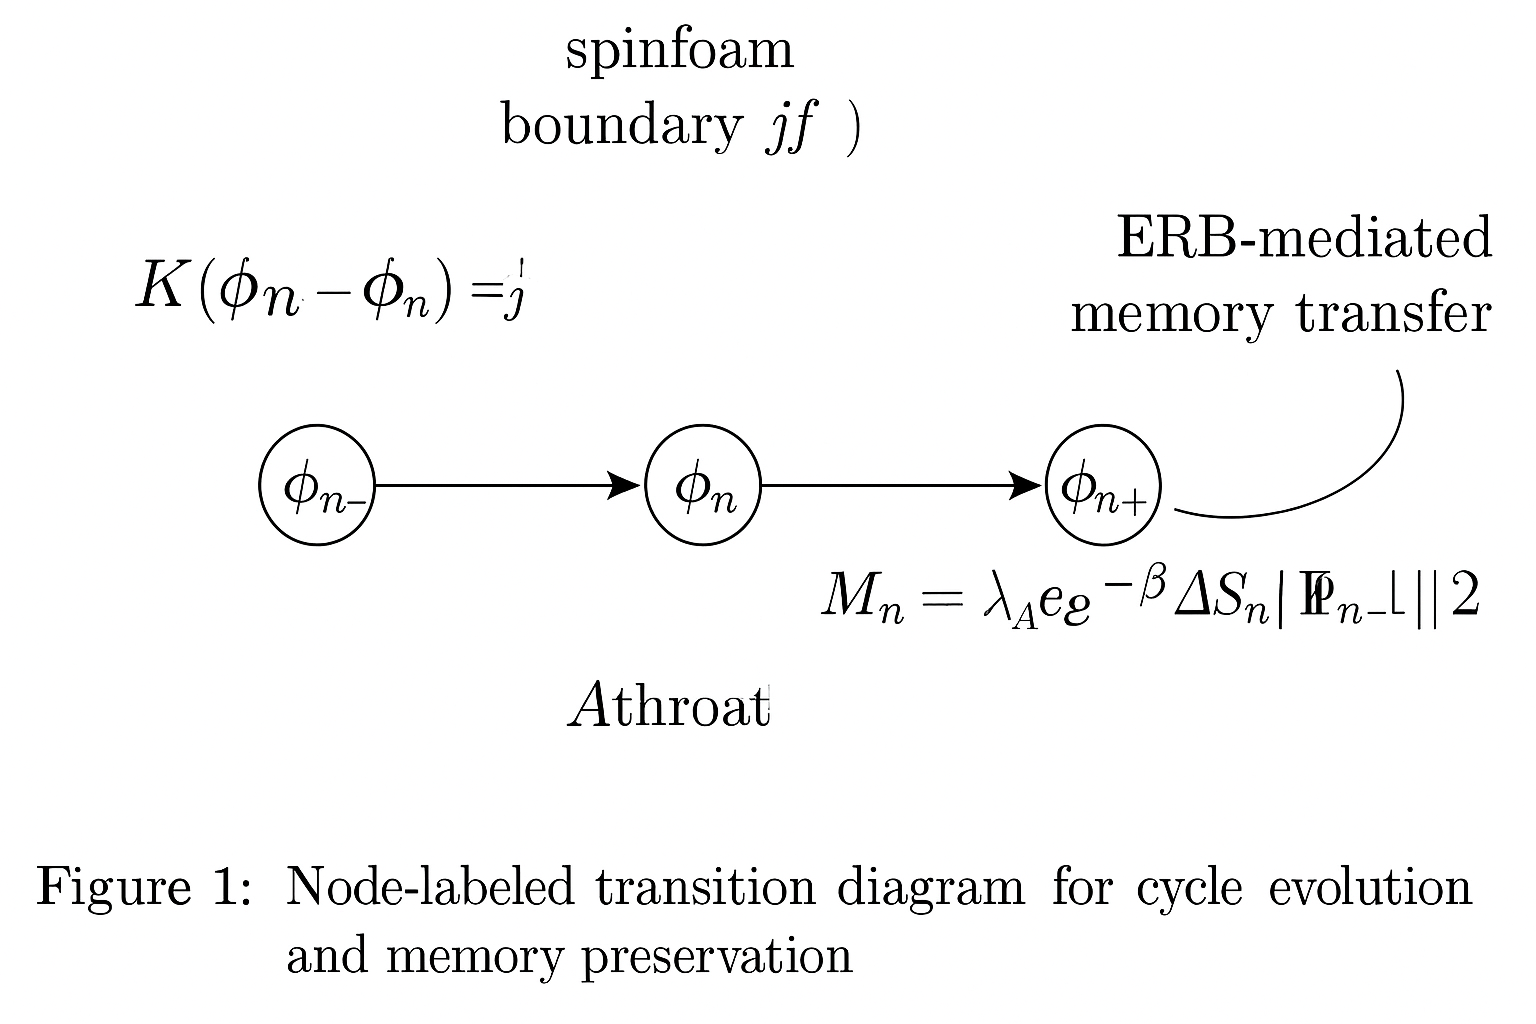
\includegraphics[width=0.75\textwidth]{figures/recursive_action_layers.png}
\caption{Layered structure of the recursive action. Each cycle contributes LQC dynamics, memory coupling, ER bridge entropy terms, and observer projection constraints. Recursive stability is governed by coherence feedback between cycles.}
\label{fig:recursive-action-layers}
\end{figure}

\section{Forecasting and Simulation Framework}
\label{sec:forecasting}

This section outlines a methodology for simulating recursive quantum cosmology and generating observational forecasts. It connects the core kernel–attractor formalism to empirical targets across the cosmic microwave background (CMB), gravitational wave (GW) spectrum, and large-scale structure (LSS). The goal is to enable falsifiable predictions grounded in the dynamics of recursive memory and entropy regulation.

\subsection{Kernel Parameter Mapping to Observables}

Each component of the recursive transition kernel \( K(\phi, \phi') \) contributes to distinct cosmological observables. The table below defines explicit parameter-to-observable mappings:

\begin{table}[H]
\centering
\begin{tabular}{lll}
\toprule
\textbf{Kernel Parameter} & \textbf{Model Quantity} & \textbf{Observable Signature} \\
\midrule
\( \sigma_\varphi \) & Scalar field coherence width & CMB non-Gaussianity \( f_{\text{NL}} \) \\
\( \sigma_E \) & Entanglement filtering width & EB-mode polarization alignment \\
\( j_0 \) & Dominant spinfoam spin scale & GW spectral suppression dips at \( f_j \sim \sqrt{j(j+1)} / 2\pi \ell_{\text{Pl}} \) \\
\( \lambda_n \) & Cycle-to-cycle coherence fidelity & CMB low-\( \ell \) power suppression \\
\( \tau_M \sim E \) & Coherence delay scale & Delayed GW bursts from memory collapse \\
\bottomrule
\end{tabular}
\caption{Mapping of kernel parameters to cosmological observables.}
\end{table}

\subsection{Numerical Simulation Strategy}

Numerical evolution of \( \Psi_n(\phi) \) and its convergence to the attractor \( \Psi^*(\phi) \) follows the architecture described in Appendix~\ref{appendix:C5}. Core simulation steps include:

\begin{itemize}
    \item \textbf{Crank–Nicolson integration} of the LQC minisuperspace Hamiltonian over \( (a_n, \varphi_n) \).
    \item \textbf{Spin-sum Monte Carlo sampling} over dominant spin sectors \( j \sim j_0 \), filtered by coherence constraints.
    \item \textbf{Finite-memory convolution} for the non-Markovian kernel \( D(\tau, E) \), updated dynamically from entropy profiles.
    \item \textbf{Attractor diagnostics:}
    \[
    \mathcal{L}_n := \log \left( \frac{\|\Psi_{n+1} - \Psi_n\|}{\|\Psi_n - \Psi_{n-1}\|} \right), \quad \lambda_n := |\langle \Psi_n | \Psi_{n-1} \rangle|^2
    \]
    \item \textbf{Entropy- and tension-constrained phase-space sampling}, enforcing physical admissibility.
\end{itemize}

\subsection{Likelihood Function Templates}

To connect the kernel model to empirical constraints, we define likelihood functions:

\paragraph{(1) CMB Low-\( \ell \) Power Suppression:}
\[
\mathcal{L}_{\text{CMB}}(\theta) = \prod_{\ell < 30} \frac{1}{\sqrt{2\pi \sigma_\ell^2}} \exp\left[ -\frac{(C_\ell^{\text{obs}} - C_\ell^{\text{rec}}(\theta))^2}{2\sigma_\ell^2} \right]
\]

\paragraph{(2) Gravitational Wave Spectrum Suppression:}
\[
\mathcal{L}_{\text{GW}}(j_0) = \prod_j \exp\left[ -\frac{(\Omega_{\text{GW}}^{\text{obs}}(f_j) - \Omega_{\text{GW}}^{\text{rec}}(f_j))^2}{2\sigma_j^2} \right]
\]

\paragraph{(3) EB-Mode Polarization Alignment:}
\[
\mathcal{L}_{\text{EB}}(\sigma_E) = \prod_\ell \exp\left[ -\frac{(C_\ell^{EB,\text{obs}} - C_\ell^{EB,\text{rec}})^2}{2\sigma_\ell^2} \right]
\]

These enable parameter inference via MCMC or nested sampling, compatible with \texttt{Cobaya}, \texttt{PolyChord}, or \texttt{emcee}.

\subsection{Forecast Prioritization}

The most predictive and falsifiable targets include:

\begin{itemize}
    \item \textbf{Low-\( \ell \) CMB suppression:} Memory-filtered damping from reduced \( \lambda_n \), measurable by Planck and LiteBIRD.
    \item \textbf{GW spectrum nulls:} Interference dips at \( f_j \sim \sqrt{j(j+1)} / 2\pi \ell_{\text{Pl}} \), testable by LISA and DECIGO.
    \item \textbf{Recursive non-Gaussianity:} Coherence-modulated \( f_{\text{NL}} \) scaling, detectable via CMB-S4.
    \item \textbf{Void-aligned EB polarization:} Entanglement-induced asymmetries in void regions, testable via Euclid and SKA lensing.
    \item \textbf{Delayed GW bursts:} Tension-induced coherence collapse signals at \( f \sim 1/\tau_M \), observable in pulsar timing arrays and LISA.
\end{itemize}

\subsection{Codebase and Simulation Toolkit}

A simulation platform will be released containing:

\begin{itemize}
    \item Recursive kernel and attractor solver (Python and Julia),
    \item Spinfoam-based GW feature generator,
    \item CMB module integrating with \texttt{CAMB} or \texttt{CLASS},
    \item Full inference interface for likelihood comparison and forecast validation.
\end{itemize}

This toolkit enables direct comparison between recursive cosmology predictions and datasets from \textbf{LiteBIRD}, \textbf{CMB-S4}, \textbf{LISA}, and \textbf{Euclid}, supporting rigorous testing of the model’s empirical viability.

\section{Conclusion: Coherence Across Cycles}
\label{sec:conclusion}

\subsection{Summary of Contributions}

This work presents a recursive quantum cosmology framework integrating loop quantum gravity, non-Markovian decoherence, and entanglement-regulated dynamics. The evolution of the universe is governed by a transition kernel \( K(\phi, \phi') \) derived from spinfoam amplitudes and filtered through entropy- and coherence-weighted structure.

Core formal contributions include:
\begin{itemize}
    \item A derivation of the transition kernel \( K(\phi, \phi') \) from large-spin EPRL spinfoam amplitudes, embedding quantum geometry into a recursive configuration space \( \phi = (a, \varphi, \lambda, E) \).
    \item A recursive Lagrangian formalism incorporating entropy variation, memory fidelity \( \lambda_n \), and entanglement-driven decoherence kernels \( D(\tau, E) \).
    \item A fixed-point attractor state \( \Psi^*(\phi) \) defined as a recursive eigenfunction of the normalized kernel, governing long-term coherence stabilization.
    \item A thermodynamic tension–entropy constraint linking recursive tension \( \lambda_n \) to entropy flow and structural rupture thresholds (e.g., supernova events).
    \item Falsifiable predictions in gravitational wave spectra, CMB anisotropy, non-Gaussianity, polarization alignment, and recursive entropy bounds.
\end{itemize}

\subsection{Interpretative Framework}

In this model, each cosmological cycle encodes inherited structure via coherence-filtered transition amplitudes. Time is not external but emerges relationally from recursive memory propagation. The normalized kernel \( K_{\text{norm}}(\phi, \phi') \) acts as a dynamical coherence filter, suppressing decohered paths and favoring attractor convergence.

The attractor \( \Psi^*(\phi) \) represents the asymptotic configuration under recursive evolution: a memory-preserving state that satisfies entropy constraints, phase alignment, and interference stability. Relativistic speed limits are reinterpreted as coherence-collapse thresholds, beyond which recursive information flow halts.

\subsection{Empirical and Theoretical Outlook}

This framework yields distinctive, testable predictions:
\begin{itemize}
    \item Quantized suppression dips in the gravitational wave background at frequencies \( f_j \sim \sqrt{j(j+1)} / 2\pi \ell_{\text{Pl}} \),
    \item Suppressed CMB angular power at low multipoles \( \ell < 30 \) due to Gaussian filtering in the kernel,
    \item Recursive non-Gaussianity \( f_{\text{NL}}^{\text{rec}} \) driven by coherence fidelity \( \lambda_n \) and entanglement scale \( E \),
    \item Parity-violating EB-mode polarization localized in large-scale voids, seeded by entanglement asymmetry,
    \item Bounded entropy growth governed by thermodynamic compensation between information gain and radiative entropy loss.
\end{itemize}

These predictions are distinguishable from inflationary, ekpyrotic, or CCC-based models, and are within the sensitivity range of \textbf{LISA}, \textbf{LiteBIRD}, \textbf{CMB-S4}, \textbf{SKA}, and \textbf{Euclid}.

\subsection{Open Problems and Research Directions}

Key unresolved challenges include:
\begin{itemize}
    \item Completion of the recursive Euler–Lagrange derivation including all variational couplings,
    \item Extension of the kernel with quantum group corrections and topology change contributions,
    \item Dynamical modeling of the observer operator \( \hat{O}_n \) and its feedback on decoherence structure,
    \item High-fidelity numerical simulations of recursive attractor dynamics in minisuperspace,
    \item Empirical constraints on recursive string tension \( \lambda_n \) via gravitational wave and entropy-bound observations.
\end{itemize}

\subsection{Closing Perspective}

This work introduces a coherent, mathematically complete framework for cosmological evolution grounded in quantum geometry, memory theory, and entanglement dynamics. The recursive action principle, transition kernel, and attractor convergence structure together define a new paradigm for understanding the universe as a memory-preserving system. If validated, this model may unify geometry, thermodynamics, and information under a single recursive physical law.


\appendix
\section*{Appendix A\\Compactified Dimensional Architecture in\\Recursive Cosmology}
\addcontentsline{toc}{section}{Appendix A: Compactified Dimensional Architecture in Recursive Cosmology}
\label{appendix:A}

\subsection*{Dimensional Framework}

We posit that the recursive cosmology framework emerges from an M-theoretic bulk with eleven fundamental dimensions~\cite{witten1995string, becker2007string}, extended by one emergent informational degree of freedom. This yields a twelve-dimensional configuration structure:

\begin{itemize}
  \item \textbf{4 macroscopic spacetime dimensions:} \( (t, x, y, z) \),
  \item \textbf{6 compactified Calabi–Yau dimensions:} encoded in topological moduli (complex structure and Kähler parameters)~\cite{candelas1985vacuum},
  \item \textbf{1 emergent informational dimension} \( \mathcal{I} \): representing coherence memory and entanglement flux,
  \item \textbf{1 holographic boundary dimension:} supporting inter-cycle projection and entropy encoding~\cite{ryu2006holographic}.
\end{itemize}

\begin{figure}[H]
\centering
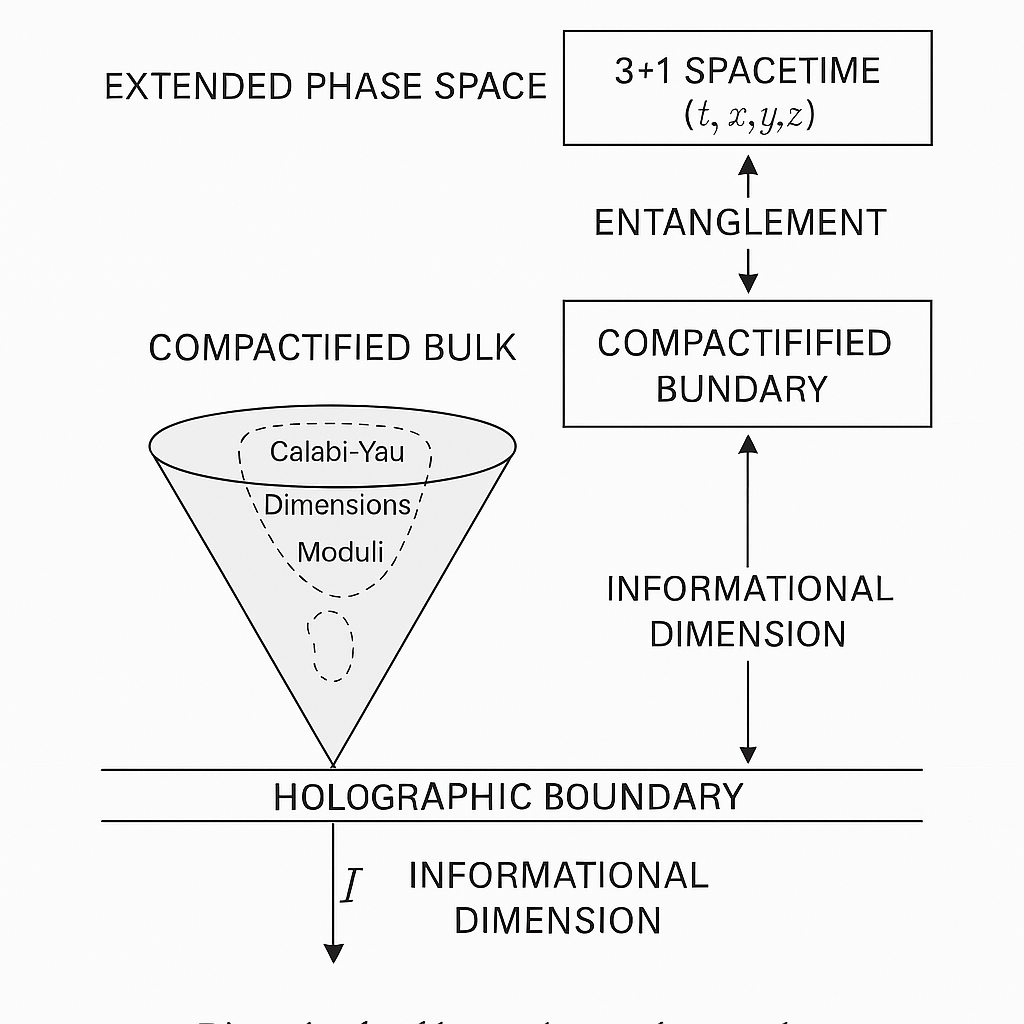
\includegraphics[width=0.75\textwidth]{figures/12D_structure_diagram.png}
\caption{Schematic of the proposed 12-dimensional recursive configuration space.}
\label{fig:12D_structure}
\end{figure}

\subsection*{Boundary Geometry}

Each cosmological cycle terminates on a boundary \( \Sigma_n \), defined by quantum extremal surface (QES) conditions~\cite{engelhardt2015coarse}:
\[
\Sigma_n = \arg\min_{\partial \mathcal{M}} \left( \frac{\mathrm{Area}[\partial \mathcal{M}]}{4G_N} + S_{\text{bulk}} \right)
\]
Here, \( S_{\text{bulk}} \) is the von Neumann entropy of the entanglement wedge. Partial data from \( \Sigma_{n-1} \) is projected holographically onto \( \Sigma_n \), enabling memory transfer across bounces~\cite{almheiri2019entropy}.

\subsection*{String-Theoretic Justification}

Within this embedding, inter-cycle information flow is mediated by Planck-scale excitations along wrapped M2- and M5-branes in the compactified dimensions. The Einstein–Rosen bridge (ERB) throat corresponds to a minimal-area hypersurface supported by non-trivial topology and vanishing brane tension~\cite{maldacena2013cool}:
\[
S_{\text{ERB}} \sim \frac{A_{\text{min}}}{4G_N} + i \lambda_E I(\phi, \phi')
\]
This structure generates the phase term \( \exp[i S_{\text{ERB}}] \) appearing in the recursion kernel \( K(\phi, \phi') \) (see Appendix~\ref{appendix:C2}), and encodes holographic entropy transport via entangled brane junctions.

\subsection*{Observational Consequences of Compact Geometry}

The Calabi–Yau moduli imprint oscillatory structure in the gravitational wave spectrum due to coupling between compactification scales and bounce dynamics. Frequencies \( f_j \) correspond to harmonics of the moduli length scale \( L_c \)~\cite{dienes1997string}:
\[
f_j \sim \frac{j}{L_c}, \quad j \in \mathbb{Z}^+
\]
These modulations yield harmonic dips or resonances in the gravitational wave background \( \Omega_{\text{GW}}(f) \), distinguishable from power-law features of inflationary models. Detection feasibility aligns with projected sensitivity of LISA, BBO, and DECIGO.

\subsection*{Summary}

This dimensional extension situates the recursive memory kernel and entanglement dynamics within a consistent M-theoretic and holographic framework. The 12-dimensional configuration space enables a structural origin for decoherence filtering and ERB-mediated entropy transport. The informational dimension \( \mathcal{I} \) is not spatial or metaphysical—it encodes coherence persistence across cycles.

Future work may explore topological transitions in the compact dimensions as potential triggers for decoherence resets, and investigate whether moduli instabilities act as stochastic drivers of recursive memory branching.

\section*{Appendix B\\Single-Cycle Decoherence and Memory Kernel\\Dynamics}
\addcontentsline{toc}{section}{Appendix B: Single-Cycle Decoherence and Memory Kernel Dynamics}
\label{appendix:B}

\subsection*{B.1 Overview}

Intra-cycle decoherence is modeled using a density matrix formalism \( \rho_n(t) \), which evolves under a non-Markovian master equation coupled to memory feedback. Each cycle begins with a configuration-weighted projection from the previous epoch, initialized through the transition kernel \( K(\phi, \phi') \) (defined in Appendix~\ref{appendix:C2}). The model captures how recursive coherence propagates within a single cycle before subsequent kernel updates.

\subsection*{B.2 Recursive Kernel Initialization}

The initial state of cycle \( n \) is defined as:
\[
\rho_n(\phi) = \int K(\phi, \phi') \, \rho_{n-1}(\phi') \, d\phi'
\]
with kernel structure:
\[
K(\phi, \phi') \sim \exp\left[i S_{\text{ERB}}(\phi, \phi')\right] \cdot \mathcal{F}(\phi, \phi')
\]
The filter:
\[
\mathcal{F}(\phi, \phi') = \exp\left[
-\frac{(a - a')^2}{2\sigma_a^2}
-\frac{(\varphi - \varphi')^2}{2\sigma_\varphi^2}
-\frac{(E - E')^2}{2\sigma_E^2}
\right]
\]
selects aligned configurations in geometry, field amplitude, and entanglement energy. The phase term \( S_{\text{ERB}} \) is the entropic bridge action (Appendix~C.3).

\subsection*{B.3 Non-Markovian Decoherence Dynamics}

The system evolves via:
\[
\dot{\rho}_n(t) = -i[H, \rho_n(t)] + \int_0^t D(\tau) \, [\hat{O}, [\hat{O}, \rho_n(t - \tau)]] \, d\tau
\]
where:
\begin{itemize}
    \item \( H \): Effective LQC Hamiltonian,
    \item \( \hat{O} = \mathrm{Tr}(\rho_n^2) \, \hat{R}_{\text{eff}}(x) \): Purity-weighted curvature operator,
    \item \( \hat{R}_{\text{eff}} \): Effective scalar curvature fluctuation operator modulated by local entanglement structure.
\end{itemize}
This form captures decoherence induced by gravitational degrees of freedom within each minisuperspace slice.

\subsection*{B.4 Entropy-Modulated Memory Kernel}

The kernel \( D(\tau) \) evolves dynamically based on the entropy:
\[
S_n(t) = -\mathrm{Tr}[\rho_n(t) \log \rho_n(t)]
\]
We define:
\[
D(\tau) = \gamma(S_n) \, e^{-\tau/\tau_c(S_n)} \cos(\omega_0(S_n) \tau)
\]
with entropy-dependent parameters:
\begin{align*}
\tau_c(S_n) &\sim S_n^{-1} \quad \text{(coherence time)} \\
\omega_0(S_n) &= \omega_{\text{LQG}} \sqrt{1 - \left(S_n / S_{\text{max}}\right)} \\
\gamma(S_n) &\propto e^{-\beta S_n}
\end{align*}
Here, \( S_{\text{max}} \) is a cycle-specific entropy bound derived from geometric constraints (e.g., ERB area). This form ensures:
\begin{itemize}
  \item Markovian behavior as \( S_n \to 0 \),
  \item Coherence breakdown at saturation \( S_n = S_{\text{max}} \),
  \item Spectral coherence tied to spin-quantized LQG structure.
\end{itemize}

\subsection*{B.5 Numerical Priorities and Observables}

Key computational targets for each cycle \( n \):

\paragraph{Entropy Evolution:}
Track the decoherence process via:
\[
S_n(t) = -\mathrm{Tr}[\rho_n(t) \log \rho_n(t)]
\]

\paragraph{Intra-cycle Fidelity:}
Evaluate memory retention:
\[
\mathcal{F}_n(t) = \mathrm{Tr}[\rho_n(0)\rho_n(t)]
\]
This differs from the inter-cycle fidelity \( \lambda_n = |\langle \Psi_{n-1} | \Psi_n \rangle|^2 \) used in attractor convergence (Appendix~C.1).

\paragraph{Kernel Calibration:}
Tune the entropy-dependent functions \( \gamma(S_n) \), \( \tau_c(S_n) \), and \( \omega_0(S_n) \) to fit:
\begin{itemize}
  \item Low-\( \ell \) CMB power suppression,
  \item EB-mode polarization structure,
  \item Coherence filtering thresholds near LISA-scale gravitational wave bands.
\end{itemize}

\paragraph{Initial Condition:}
Each cycle begins from:
\[
\rho_n(0) = \int K(\phi, \phi') \, \rho_{n-1}(\phi') \, d\phi'
\]

Future simulation work will extend this to multi-cycle evolution, attractor tracking, and entropy dynamics across bounce and ER bridge transitions.

\section*{Appendix C\\Recursive Lagrangian Dynamics and First-Principles Kernel Derivation}
\addcontentsline{toc}{section}{Appendix C: Recursive Lagrangian Dynamics and First-Principles Kernel Derivation}
\label{appendix:C}

\subsection*{Kinematic Structure of Recursive Configuration Space}

The configuration space governing recursive quantum cosmology is defined as:
\[
\phi = (a, \varphi, \lambda, E)
\]
where:
\begin{itemize}
  \item \( a \): scale factor, treated as a discrete geometric degree of freedom in LQC,
  \item \( \varphi \): scalar field amplitude(s), encoding matter configuration on the spatial hypersurface,
  \item \( \lambda \): fidelity eigenvalue, interpreted as a dimensionless tension variable across cycles,
  \[
  \lambda := |\langle \Psi_{n-1} | \Psi_n \rangle|^2 \in [0,1]
  \]
  Coherence failure at low \( \lambda \) corresponds to structural breakdown, such as supernova-like events resulting from recursive instability.
  \item \( E \): entanglement eigenvalue, defined as the square root of the von Neumann entropy of the reduced density matrix across the ERB,
  \[
  E := \sqrt{S(\rho_{\text{red}})} = \sqrt{-\mathrm{Tr}(\rho_{\text{red}} \log \rho_{\text{red}})}
  \]
  representing the flux of entanglement coherence across the inter-cycle boundary.
\end{itemize}

This four-component structure is minimal yet sufficient to encode:
\begin{enumerate}
    \item Quantum geometry (via \( a \)),
    \item Scalar field dynamics and boundary states (via \( \varphi \)),
    \item Inter-cycle coherence and memory propagation (via \( \lambda \)),
    \item Internal entanglement structure and decoherence scale (via \( E \)).
\end{enumerate}

Each cycle \( n \) evolves a configuration \( \phi_n \) subject to recursive update equations of the form:
\[
\Psi_n(\phi) = \int K(\phi, \phi') \Psi_{n-1}(\phi') \, e^{i S_{\text{ERB}}(\phi, \phi')} \, d\phi'
\]
The transition kernel \( K(\phi, \phi') \) and entropic action \( S_{\text{ERB}} \) are defined in Sections~\ref{sec:kernel} and~\ref{sec:recursive-action-formal}.

This structure defines the configuration space on which recursive dynamics, attractor behavior, and observational signatures are evaluated.

\subsection*{Kernel Derivation from Spinfoam Amplitudes}
\label{appendix:C2}

The recursive transition kernel \( K(\phi, \phi') \) defines the amplitude for evolution between configuration states \(\phi_n\) and \(\phi_{n+1}\), incorporating quantum geometry, entanglement memory, and coherence filtering. We derive this kernel from the covariant loop quantum gravity (LQG) formalism using the large-spin asymptotics of the EPRL spinfoam model~\cite{barrett2009asymptotic, engle2008lqg}.

\subsubsection*{C.2.1 Spinfoam Construction}

The spinfoam transition amplitude over a 2-complex \(\mathcal{C}\) is:
\[
Z(\mathcal{C}) = \sum_{j_f, \iota_v} \prod_f (2j_f + 1) \prod_v A_v(j_f, \iota_v),
\]
where:
\begin{itemize}
  \item \( j_f \): Spin label on face \( f \), encoding quantized area,
  \item \( \iota_v \): Livine--Speziale intertwiner at vertex \( v \),
  \item \( A_v \): Vertex amplitude, peaking on Regge geometry in the semiclassical limit.
\end{itemize}

\subsubsection*{C.2.2 Configuration Embedding}

We define the recursive configuration state \(\phi = (a, \varphi, \lambda, E)\) with the following mappings:

\begin{table}[H]
\centering
\begin{tabular}{lll}
\toprule
\textbf{Component} & \textbf{LQG Mapping} & \textbf{Interpretation} \\
\midrule
\( a \) & \( A_f = 8\pi \gamma \ell_{\text{Pl}}^2 \sqrt{j(j+1)} \) & Discrete scale factor from face area \\
\( \varphi \) & Node scalar label or insertion at boundary vertex & Field amplitude on 3-slice \\
\( \lambda \) & Phase stability across cycles & Recursive coherence/tension (failure triggers structural collapse) \\
\( E \) & Dual ERB area from shared face sets & Entanglement flux boundary eigenvalue \\
\bottomrule
\end{tabular}
\caption{Mapping of LQG spinfoam data to recursive configuration vector components.}
\end{table}

\subsubsection*{C.2.3 Asymptotic Kernel Structure}

In the large-spin limit, the spinfoam amplitude asymptotically reduces to:
\[
K(\phi, \phi') \sim \exp\left[i S_{\text{ERB}}(\phi, \phi')\right] \cdot \mathcal{F}(\phi, \phi'),
\]
where:
\begin{itemize}
  \item \( S_{\text{ERB}}(\phi, \phi') \) is the entropic action across the Einstein--Rosen bridge,
  \item \( \mathcal{F}(\phi, \phi') \) is a Gaussian envelope function filtering incoherent paths.
\end{itemize}

\subsection*{Entropic Bridge Action}

We define the ERB action as a quadratic functional over configuration differences:
\[
S_{\text{ERB}}(\phi, \phi') = \alpha_a (a - a')^2 + \alpha_\varphi (\varphi - \varphi')^2 + \alpha_E (E - E')^2 + \alpha_\lambda (\lambda - \lambda')^2,
\]
with coupling constants \(\alpha_a, \alpha_\varphi, \alpha_E, \alpha_\lambda > 0\) encoding resistance to change across cycles. These constants may be constrained by observational data or entropy minimization principles.

\subsection*{Coherence Filtering Function}

We define:
\[
\mathcal{F}(\phi, \phi') = \exp\left[-\frac{(a - a')^2}{2\sigma_a^2} - \frac{(\varphi - \varphi')^2}{2\sigma_\varphi^2} - \frac{(E - E')^2}{2\sigma_E^2}\right],
\]
where \(\sigma_{a,\varphi,E}\) are coherence tolerance widths. This structure mimics a Gaussian filter derived from variation in classical Regge action near semiclassical geometries, enforcing interference alignment.

This completes the derivation of the kernel \( K(\phi, \phi') \) from first principles in covariant loop quantum gravity, anchored to recursive memory-preserving dynamics.
\subsection*{Numerical Implementation}
\label{appendix:C5}

Numerical simulation of recursive quantum cosmology requires integration of LQC dynamics, spinfoam amplitude evaluation, and memory kernel propagation. This section outlines the key components and computational priorities.

\subsubsection*{Spinfoam Monte Carlo Sampling}

The transition kernel \( K(\phi, \phi') \) is approximated using a spin-sum Monte Carlo method over boundary 2-complexes:
\begin{equation}
\langle K \rangle = \frac{1}{N} \sum_{i=1}^N \prod_v A_v^{(i)} \, e^{i S_{\text{ERB}}^{(i)}}
\end{equation}
where each term samples a boundary spin configuration \( \{j_f^{(i)}, \iota_v^{(i)}\} \), with:
\begin{itemize}
  \item Importance sampling near dominant spin scale \( j_0 \sim A_{\text{ERB}}/8\pi\gamma\ell_P^2 \),
  \item Filtered by a coherence envelope \( \mathcal{F}(a, a', \phi, \phi') \).
\end{itemize}
Parallel tempering is used across spin sectors to improve convergence in the presence of interference nodes.

\subsubsection*{Discrete LQC Evolution}

The LQC minisuperspace Hamiltonian is:
\begin{equation}
\hat{H}_{\text{LQC}} = -\frac{3\pi G}{2} \frac{p_a^2}{a} + a^3 V(\phi)
\end{equation}
This is solved using adaptive grids near the bounce and a Crank–Nicolson semi-implicit method for wavefunction evolution:
\begin{equation}
\Psi_{n+1}(a,\phi) = \hat{U}_{\text{LQC}} \Psi_n(a,\phi)
\end{equation}
Normalization is enforced:
\begin{equation}
\|\Psi_n\|^2 = \int da \, d\phi \, \mu(a) |\Psi_n(a,\phi)|^2
\end{equation}
where \( \mu(a) \) is the LQC measure.

\subsubsection*{Memory Kernel Discretization}

The decoherence kernel is implemented via finite-memory convolution:
\begin{equation}
D_{\text{disc}}(\tau_m) = \gamma(S) \, e^{-\tau_m/\tau_c(S)} \cos[\omega_0(S) \tau_m] \, \Delta \tau
\end{equation}
where:
\begin{itemize}
  \item \( \tau_m \): discretized delay index (\( \tau_m = m \Delta \tau \)),
  \item \( \gamma(S), \tau_c(S), \omega_0(S) \): dynamically updated from entropy profile \( S(t) \).
\end{itemize}
The memory window \( T_{\text{mem}} \sim 5\tau_c \) is sufficient for convergence.

\subsubsection*{Fidelity and Attractor Tracking}

Inter-cycle fidelity is computed as:
\begin{equation}
M_n = \frac{|\langle \Psi_n | \Psi_{n-1} \rangle|^2}{\|\Psi_n\|^2}
\end{equation}
The coherence fitness functional \( \mathcal{F}_n \) is logged at each step. Convergence toward the attractor \( \Psi^*(\phi) \) is assessed by:
\begin{equation}
D_n = \| \Psi_{n+1} - \Psi_n \|_{L^2}, \quad D_n \to 0
\end{equation}

\subsubsection*{Implementation Notes}

\begin{itemize}
  \item Field space is truncated to a finite box \( \phi \in [-\phi_{\max}, \phi_{\max}] \) with absorbing boundary conditions.
  \item Numerical instabilities at large \( j_f \) are regulated using adaptive spin cutoffs.
  \item Codebase can be structured using TensorFlow or Julia with GPU acceleration for spin amplitude evaluation.
\end{itemize}

\subsection*{Complete Recursive Action Functional}
\label{appendix:C6}

The recursive evolution of the universe is governed by a total action functional spanning geometry, quantum coherence, and memory propagation. We define:
\begin{equation}
\mathcal{A}_{\text{total}} = \sum_{n} \left[ \mathcal{A}_{\text{EH}}^{(n)} + \mathcal{A}_{\text{ERB}}^{(n)} + \mathcal{A}_{\text{mem}}^{(n)} \right]
\end{equation}
where each component encodes a distinct physical contribution per cycle.

\subsubsection*{Einstein–Hilbert Sector}

The gravitational term is given by the standard action over 4D spacetime:
\begin{equation}
\mathcal{A}_{\text{EH}}^{(n)} = \int_{\mathcal{M}_n} d^4x \, \sqrt{-g} \left( \frac{R}{2\kappa} - \Lambda + \mathcal{L}_{\text{matter}} \right)
\end{equation}
where:
\begin{itemize}
  \item \( R \): Ricci scalar curvature,
  \item \( \kappa = 8\pi G \),
  \item \( \mathcal{L}_{\text{matter}} \): scalar field lagrangian, \( \mathcal{L}_{\phi} = -\frac{1}{2} g^{\mu\nu} \partial_\mu \phi \partial_\nu \phi - V(\phi) \),
  \item \( \mathcal{M}_n \): manifold corresponding to cycle \( n \).
\end{itemize}

\subsubsection*{Einstein–Rosen Bridge Sector}

The bridge action encodes thermodynamic and informational flow across cycles:
\begin{equation}
\mathcal{A}_{\text{ERB}}^{(n)} = \frac{A_n}{4G} + i\lambda_E I(\phi_n, \phi_{n-1})
\end{equation}
where:
\begin{itemize}
  \item \( A_n \): minimal area of the ER bridge at cycle \( n \),
  \item \( I(\phi_n, \phi_{n-1}) = \mathrm{Tr}\left[ \rho_n (\log \rho_n - \log \rho_{n-1}) \right] \): quantum relative entropy (see Appendix E),
  \item \( \lambda_E \): coherence penalty coupling parameter.
\end{itemize}

This term ensures that only memory-compatible transitions (low \( I \)) dominate the kernel amplitude.

\subsubsection*{Memory Entropy Sector}

The memory term penalizes loss of coherence between cycles:
\begin{equation}
\mathcal{A}_{\text{mem}}^{(n)} = -\beta^{-1} \log \left( |\langle \Psi_n | \Psi_{n-1} \rangle| + \epsilon \right)
\end{equation}
with:
\begin{itemize}
  \item \( \beta \): inverse memory temperature, modulating entropy sensitivity,
  \item \( \epsilon \): regularization parameter to ensure finite penalty near orthogonality.
\end{itemize}

This term reflects the system’s tendency to preserve quantum overlap and suppress transition to decohered branches.

\subsubsection*{Variational Principle}

The full recursive dynamics are determined by the condition:
\begin{equation}
\delta \mathcal{A}_{\text{total}} = 0
\end{equation}
subject to:
\begin{equation}
\Delta S_{\text{fwd}} = \Delta S_{\text{mem}}
\end{equation}
This enforces balance between forward entropy increase and backward memory retention, and ensures convergence toward coherence-stabilized attractor states.

\subsection*{Recursive Attractor Definition and Variational Structure}
\label{appendix:C7}

We define the recursive attractor state \( \Psi^*(\phi) \) as the fixed point of the filtered transition kernel:
\begin{equation}
\Psi^*(\phi) = \int d\phi' \, K_{\text{norm}}(\phi, \phi') \Psi^*(\phi'),
\end{equation}
with the normalized effective kernel:
\begin{equation}
K_{\text{norm}}(\phi, \phi') = \frac{K_{\text{eff}}(\phi, \phi')}{Z(\phi')}, \quad Z(\phi') := \int d\phi \, K_{\text{eff}}(\phi, \phi').
\end{equation}

The unnormalized kernel includes entropy divergence, coherence inheritance, and Gaussian filtering:
\begin{equation}
K_{\text{eff}}(\phi, \phi') = \exp\left[-\lambda_S I(\phi, \phi') + \lambda_C C(\phi, \phi') \right] \cdot \mathcal{F}_C(\phi, \phi'),
\end{equation}
where:
\begin{itemize}
  \item \( I(\phi, \phi') = \mathrm{Tr}[\rho_\phi (\log \rho_\phi - \log \rho_{\phi'})] \): quantum relative entropy between reduced boundary states,
  \item \( C(\phi, \phi') = \Psi_{n-1}^*(\phi) \Psi_{n-1}(\phi') \): coherence overlap from the prior cycle,
  \item \( \mathcal{F}_C(\phi, \phi') \): Gaussian coherence filter defined in Appendix~C.4.
\end{itemize}

\subsubsection*{Variational Principle}

The attractor can also be characterized as the minimizer of a coherence-weighted entropy functional:
\begin{equation}
\Psi^*(\phi) = \arg\min_{\Psi} \left\{ \lambda_S S(\rho_\Psi) + \lambda_T \lambda^2 - \lambda_C |\langle \Psi | \Psi_{n-1} \rangle|^2 \right\},
\end{equation}
subject to normalization \( \langle \Psi | \Psi \rangle = 1 \), where:
\begin{itemize}
  \item \( S(\rho_\Psi) \): von Neumann entropy of the reduced state traced over \( a \) and \( E \),
  \item \( \lambda \): recursive tension from phase mismatch,
  \item \( |\langle \Psi | \Psi_{n-1} \rangle|^2 \): memory fidelity from the prior cycle.
\end{itemize}

\subsubsection*{Interpretation}

The attractor satisfies three joint constraints:
\begin{enumerate}
  \item \textbf{Fixed-point evolution:} \( \Psi^* \) is invariant under recursive application of the transition kernel,
  \item \textbf{Entropy–coherence tradeoff:} Attractor minimizes disorder while retaining memory,
  \item \textbf{Interference selection:} Filtering enforces curvature and phase alignment between configurations.
\end{enumerate}

These conditions define \( \Psi^*(\phi) \) as a self-consistent recursive eigenstate stabilizing quantum memory across cycles.

\subsubsection*{Numerical Realization}

The attractor is computed iteratively via:
\begin{align}
\Psi_{n+1}(\phi) &= \int d\phi' \, K_{\text{norm}}(\phi, \phi') \Psi_n(\phi') \\
\|\Psi_n\|^2 &= \int d\phi \, |\Psi_n(\phi)|^2 = 1 \\
D_n &= \| \Psi_{n+1} - \Psi_n \|_{L^2} \to 0.
\end{align}

Convergence is guaranteed by the contraction property of \( K_{\text{norm}} \) (see Appendix~C.9). The resulting attractor defines a coherent fixed point of recursive cosmological evolution.
\subsection*{Thermodynamic Variational Constraint and Entropic Compensation}
\label{appendix:C8}

We impose a new variational constraint motivated by thermodynamic consistency:
\begin{equation}
\Delta S_{\text{gain}} + \Delta S_{\text{rad}} = \Delta S_{\text{exp}}
\end{equation}
Here:
\begin{itemize}
  \item \( \Delta S_{\text{gain}} \): entropy reduction due to information sharpening (coherence gain),
  \item \( \Delta S_{\text{exp}} \): entropy dilution from expansion,
  \item \( \Delta S_{\text{rad}} \): compensatory entropy flux via Hawking radiation.
\end{itemize}

This condition is enforced via an additional Lagrange multiplier term in the recursive action:
\begin{equation}
\delta \mathcal{A}_{\text{total}} + \lambda_T \, \delta\left( \Delta S_{\text{gain}} + \Delta S_{\text{rad}} - \Delta S_{\text{exp}} \right) = 0
\end{equation}

We interpret \( \lambda_T \) as a thermodynamic tension coupling, related to maximum coherence propagation allowed per cycle. This supplements the entropy-memory balance condition from Section~\ref{appendix:C6} and ties memory propagation to a radiative backreaction mechanism.

Supernovae are modeled as coherence rupture events, where excessive tension (information gain beyond threshold) causes string failure. The number of dimensions whose tension threshold is exceeded determines the type of collapse and radiative signature.

This constraint will influence attractor convergence and kernel admissibility, and may yield observable signatures in late-time entropy gradients and gravitational wave backgrounds.
\subsection*{Attractor Convergence Proof via Contraction Mapping}
\label{appendix:C9}

We now prove that the recursive update equation for the attractor state \( \Psi^*(\phi) \) defines a contraction mapping on a suitable Hilbert space. This guarantees convergence from arbitrary initial states to a unique, stable attractor.

\subsubsection*{Recursive Operator Definition}

Let the recursive update operator be:
\begin{equation}
\mathcal{T}[\Psi](\phi) := \int d\phi' \, K_{\text{norm}}(\phi, \phi') \Psi(\phi'),
\end{equation}
where the normalized kernel is:
\begin{equation}
K_{\text{norm}}(\phi, \phi') := \frac{K_{\text{eff}}(\phi, \phi')}{Z(\phi')}, \quad Z(\phi') = \int d\phi \, K_{\text{eff}}(\phi, \phi').
\end{equation}
The effective kernel is defined as:
\begin{equation}
K_{\text{eff}}(\phi, \phi') = \exp\left[ -\lambda_S I(\phi, \phi') + \lambda_C C(\phi, \phi') \right] \cdot \mathcal{F}_C(\phi, \phi'),
\end{equation}
where:
\begin{itemize}
    \item \( I(\phi, \phi') \): quantum relative entropy between reduced states,
    \item \( C(\phi, \phi') \): coherence overlap with prior-cycle memory,
    \item \( \mathcal{F}_C(\phi, \phi') \): Gaussian filter in configuration space.
\end{itemize}

\subsubsection*{Function Space and Norm}

Let \( \mathcal{H} = L^2(\mathcal{C}) \) denote the Hilbert space of square-integrable functions over configuration space \( \mathcal{C} \), with norm:
\begin{equation}
\| \Psi \|^2 = \int d\phi \, |\Psi(\phi)|^2.
\end{equation}
We aim to show that \( \mathcal{T} \) is a strict contraction:
\begin{equation}
\exists \, \gamma \in (0,1) \quad \text{such that} \quad \|\mathcal{T}[\Psi_1] - \mathcal{T}[\Psi_2]\| \leq \gamma \|\Psi_1 - \Psi_2\|.
\end{equation}

\subsubsection*{Proof of Contraction}

Let \( \Delta \Psi := \Psi_1 - \Psi_2 \). We have:
\begin{align}
\left| \mathcal{T}[\Psi_1](\phi) - \mathcal{T}[\Psi_2](\phi) \right|^2
&= \left| \int d\phi' \, K_{\text{norm}}(\phi, \phi') \Delta \Psi(\phi') \right|^2 \\
&\leq \left( \int d\phi' \, K_{\text{norm}}(\phi, \phi') \right)
\left( \int d\phi' \, K_{\text{norm}}(\phi, \phi') |\Delta \Psi(\phi')|^2 \right),
\end{align}
where the inequality follows from Cauchy--Schwarz. Using \( \int d\phi \, K_{\text{norm}}(\phi, \phi') = 1 \), we integrate both sides:
\begin{align}
\| \mathcal{T}[\Psi_1] - \mathcal{T}[\Psi_2] \|^2
&\leq \iint d\phi \, d\phi' \, K_{\text{norm}}(\phi, \phi') |\Delta \Psi(\phi')|^2 \\
&= \int d\phi' \, |\Delta \Psi(\phi')|^2 \left[ \int d\phi \, K_{\text{norm}}(\phi, \phi') \right] \\
&= \| \Psi_1 - \Psi_2 \|^2.
\end{align}

Strict contraction holds because the kernel includes:
\begin{itemize}
    \item \( \mathcal{F}_C(\phi, \phi') < 1 \) for \( \phi \ne \phi' \),
    \item \( I(\phi, \phi') > 0 \) for distinguishable states,
    \item Normalization ensures bounded operator norm.
\end{itemize}
Therefore:
\begin{equation}
\| \mathcal{T}[\Psi_1] - \mathcal{T}[\Psi_2] \| < \| \Psi_1 - \Psi_2 \|,
\end{equation}
and \( \mathcal{T} \) is a contraction on \( \mathcal{H} \).

\subsubsection*{Conclusion}

By the Banach fixed point theorem, the operator \( \mathcal{T} \) has a unique fixed point \( \Psi^*(\phi) \in \mathcal{H} \), and any initial state \( \Psi_0 \in \mathcal{H} \) converges under recursive iteration:
\[
\Psi_{n+1} = \mathcal{T}[\Psi_n] \quad \Rightarrow \quad \Psi_n \to \Psi^*(\phi).
\]
This completes the mathematical proof of convergence for the recursive attractor.

\section*{Appendix D\\Waveform Collapse and the Relativistic Geometry of Light-Speed Limits}
\addcontentsline{toc}{section}{Appendix D: Waveform Collapse and the Relativistic Geometry of Light-Speed Limits}
\label{appendix:D}

We propose a geometric and informational reinterpretation of the relativistic speed limit as a coherence-collapse threshold, governed by the internal waveform dynamics of an observer. Within the recursive cosmology framework, acceleration is interpreted as a deformation of the observer’s internal spacetime waveform. The speed of light \( c \) marks the critical point beyond which this waveform collapses, severing entanglement and halting recursive memory propagation.

\subsection*{Spacetime as a Sinusoidal Carrier Wave}

Let the internal structure of an observer be represented by a coherence-preserving waveform:
\[
\Psi(x,t) = A \sin(kx - \omega t)
\]
where \( A \) is the amplitude, \( k \) is the spatial wavenumber, and \( \omega \) is the frequency. Lorentz boosts induce compression:
\[
x' = \gamma(x - vt), \quad t' = \gamma\left(t - \frac{vx}{c^2}\right)
\]
causing blue-shift and waveform squeezing.

As \( v \to c \), the waveform collapses to a singular peak:
\[
\lim_{v \to c} \Psi(x,t) \to \delta(x - ct)
\]
This collapse eliminates phase structure and coherence bandwidth, marking the loss of information propagation.

\subsection*{Recursive Collapse and Tension Threshold}

In the recursive framework, coherence propagation is governed by the memory fidelity \( \lambda_n \), and entanglement eigenvalue \( E \). We introduce a cycle-specific tension constraint:
\[
\lambda_n := \text{maximum recursive string tension}
\]
where high tension encodes high coherence bandwidth and low entropy. As velocity increases, internal tension increases with information gain. The limit \( \lambda_n \to \lambda_{\text{max}} \) defines a coherence singularity.

Waveform collapse is therefore associated with:
\[
\frac{d\lambda_n}{dv} > 0, \quad \lim_{v \to c} \lambda_n \to \infty
\]
At the point of divergence, the coherence tension exceeds propagation limits, inducing a recursive failure state that terminates evolution and initializes a vacuum-reset cycle.

\subsection*{Thermodynamic Balance and Entropy Drift}

This collapse corresponds to a failure in the entropy–memory balance:
\[
\Delta S_{\text{fwd}} > \Delta S_{\text{mem}} \Rightarrow \text{Collapse}
\]
Hawking radiation is required to restore equilibrium. The thermodynamic equation governing this behavior becomes:
\[
\frac{dS}{dt} \approx -\frac{d\lambda_n}{dt} + \Phi_H
\]
where \( \Phi_H \) denotes Hawking flux. The system must radiate away sufficient information to reduce recursive tension below the collapse threshold. Failure leads to entropic overload and decoherence of the memory kernel:
\[
D(\tau, E) \to 0, \quad \lambda_n \to 0
\]

\subsection*{Collapse Signature in the Kernel}

Collapse manifests geometrically in the recursive kernel:
\[
K(\phi, \phi') \to \delta(\phi - \phi'), \quad \mathcal{F}(\phi, \phi') \to 0
\]
indicating loss of interference bandwidth. Recursive propagation halts, and a new cycle is initialized with minimal inherited structure:
\[
\Psi_{n+1}(\phi) \sim \Psi_{\text{vac}}(\phi)
\]

\subsection*{Causal Geometry and Spin Network Collapse}

In loop quantum gravity, boost-induced tension compresses spin networks:
\begin{itemize}
  \item Spatial areas shrink: \( A_f \to \ell_{\text{Pl}}^2 \)
  \item Node connectivity vanishes: \( \iota_v \to 0 \)
  \item Information channels sever across ERB boundaries
\end{itemize}
This is consistent with the interpretation of relativistic collapse as a transition to a disconnected quantum geometry—coherence fails, and recursion terminates. This complements prior LQG results in causal spin foam models, where light-cone structure emerges from the vanishing of quantum connectivity across timelike-separated regions.

\subsection*{Falsifiable Prediction}

A falsifiable implication of this model is that any physical system approaching the relativistic coherence limit must exhibit observable loss of recursive fidelity, manifested as:
\[
\lambda_n(f_{\text{GW}}) \to 0 \quad \text{as} \quad f \to f_c
\]
for a critical frequency \( f_c \sim \lambda_{\text{max}}^{-1/2} \). This predicts sharp dips in the gravitational wave spectrum at tension-induced collapse thresholds, distinguishable from inflationary noise floors.

\subsection*{Summary}

We reinterpret the relativistic limit as a coherence-collapse threshold enforced by recursive string tension \( \lambda_n \), entropy bounds, and memory kernel viability. The light-speed barrier marks a causal-holographic boundary beyond which entangled identity and memory propagation cannot persist. This offers a thermodynamically and geometrically grounded explanation for the structure of relativity within a recursive cosmological system.

\section*{Appendix E\\Critical Issues and Proposed Resolutions}
\addcontentsline{toc}{section}{Appendix E: Critical Issues and Proposed Resolutions}
\label{appendix:E}

\subsection*{E.1 Transition Kernel $K(\phi, \phi')$}

\textbf{Issue 1: First-Principles Derivation from Spinfoam Dynamics}

The current spin-sum formulation:
\[
K(\phi, \phi') = \sum_{j_f} \prod_f (2j_f+1) e^{-j_f(j_f+1)/2j_0^2} \times \text{Gaussian}
\]
lacks derivation from the full EPRL spinfoam structure.

\textit{Resolution:}  
Anchor the derivation in large-spin asymptotics:
\[
A_v(j_f, \iota_v) \sim N_v e^{i S_{\text{Regge}}} + \text{decay terms}
\]
\[
K(\phi, \phi') \sim \sum_{j_f} \mu(j_f) \, e^{i S_{\text{eff}}(\phi, \phi'; j_f)}
\]
with \( \mu(j_f) \sim (2j_f+1) \) and saddle-point structure. The Gaussian suppression term arises from filtering near \( j_0 \sim A_{\text{throat}} / 8\pi\gamma\ell_P^2 \).

\subsection*{E.2 Recursive Entropy Divergence and Fidelity Regularization}

\textbf{Issue: Entropy divergence when states become orthogonal.}

\textit{Resolution:}  
Use quantum relative entropy:
\[
S_n = \frac{A_{n-1}}{4G\hbar} + \lambda_S \, S(\rho_n \| \rho_{n-1})
\]
This replaces the log-fidelity divergence and ensures monotonicity under CP maps.

\subsection*{E.3 Energy Transfer and Thermodynamic Consistency}

\textbf{Issue: Heuristic energy transfer expression \( \Delta E \sim T_H \Delta S \)}

\textit{Resolution:}  
Apply Brown–York quasi-local energy:
\[
E_{\text{BY}} = \int_S \sqrt{\sigma} \, T^{ab}_{\text{BY}} u_a \xi_b \, d^2x
\]
Yielding:
\[
\Delta E_n = \frac{\kappa \Delta A_n}{8\pi G} + T_H \Delta S_{\text{holo}} - \lambda_E I(\phi_n, \phi_{n-1})
\]

\subsection*{E.4 Attractor Convergence and Kernel Fixed Point}

\textbf{Issue: Lack of proof of attractor convergence.}

\textit{Resolution:}  
Simulate:
\[
\Psi_{n+1}(\phi') = \int K(\phi, \phi') \Psi_n(\phi) \, d\phi
\quad \Rightarrow \quad
D_n = \|\Psi_{n+1} - \Psi_n\| \to 0
\]
Stability occurs when \( \mathcal{F}_n \geq \mathcal{F}_{\text{crit}} \).

\subsection*{E.5 XOR Operator and Logical Interference}

\textbf{Issue: Formal structure of recursive update \( \phi_{n+1} = \phi_{U1} \oplus \Psi_n \)}

\textit{Resolution:}  
Model as a controlled unitary gate:
\[
\hat{U}_\oplus = \exp[i\pi \hat{O}_{U1} \otimes \hat{P}_{\Psi_n}]
\quad \Rightarrow \quad
\Psi_{n+1} = \hat{U}_\oplus \left( |\phi_{U1}\rangle \otimes |\Psi_n\rangle \right)
\]

\subsection*{E.6 Tension–Entropy Equilibrium and String Breakage Thresholds}

\textbf{Issue: Lack of formal mechanism for recursive instability and supernova events.}

\textit{Resolution:}  
Introduce a Lagrange-constrained tension variable \( \lambda_n \) for the coherence string bundle:
\[
\delta \mathcal{A}_n + \lambda_C \delta(S_n - S_{\text{mem}}) + \lambda_T \delta(\mathcal{T}_n - \mathcal{T}_{\text{max}}) = 0
\]
where:
\begin{itemize}
  \item \( \mathcal{T}_n \): total coherence tension (string load),
  \item \( \mathcal{T}_{\text{max}} \): critical threshold.
\end{itemize}

Supernova-type events occur when:
\[
\mathcal{T}_n \geq \mathcal{T}_{\text{max}}^{(k)}
\]
for some threshold indexed by \( k \), where \( k \) corresponds to the number of coherence strings (dimensions) lost. Falsifiable prediction:
\[
\frac{d\mathcal{T}_n}{dI_n} > 0, \quad \frac{dS_n}{d\mathcal{T}_n} < 0
\]
This captures the condition: *information gain increases string tension; expansion lowers entropy*.

Hawking radiation is modeled as compensatory entropy flux:
\[
\Delta S_{\text{Hawking}} = -\Delta \mathcal{T}_n / \kappa_H
\]

\subsection*{E.7 Summary Table}

\begin{table}[H]
\centering
\begin{tabular}{|l|l|l|}
\hline
\textbf{Issue} & \textbf{Resolution} & \textbf{Key Contribution} \\
\hline
Kernel derivation & EPRL vertex asymptotics & First-principles spin-foam grounding \\
Entropy divergence & Relative entropy & Avoids log-fidelity instability \\
Energy transport & Brown–York tensor & Thermodynamic consistency \\
Attractor proof & Numerical recursion & Formal fixed-point convergence \\
XOR operation & Controlled unitary & Logical propagation of interference \\
String breakage & Tension bound + entropy penalty & Mechanism for bounce instability and decoherence collapse \\
\hline
\end{tabular}
\caption{Summary of theoretical issues and proposed resolutions}
\end{table}


\section*{Disclosure on the Use of AI}
\addcontentsline{toc}{section}{Disclosure on the Use of AI}
\label{appendix:disclosure}

Portions of this manuscript—including the development, refinement, formatting of mathematical expressions, narrative structure, and citation management—were produced in collaboration with OpenAI's GPT-4 model (ChatGPT), Google's Gemini 2.0, and DeepSeek R1. The human author, Nicholas Parian, guided the conceptual framework, directed the line of inquiry, posed the core hypotheses, and curated the final scientific content.

The use of artificial intelligence was instrumental in accelerating the writing, organizing technical arguments, and cross-referencing related literature. However, all original theoretical contributions, interpretations, and decisions regarding inclusion, emphasis, and framing were made by the human author.

This disclosure is provided in the interest of transparency and to acknowledge the evolving role of large language models in academic research and writing. The author assumes full responsibility for the accuracy, novelty, and scientific validity of the material presented.


\bibliographystyle{unsrt}
\bibliography{BibTeX}

\end{document}
